\documentclass[11pt]{extarticle}
\usepackage{microtype}
\usepackage{fullpage}
\usepackage[ampersand]{easylist}
\ListProperties(Hide=10, Style*=$\bullet\;\,$, Style2*=$\;\,${\tiny$\blacksquare$}$\;\,$,Space*=1mm,Space2*=0.1mm)

\usepackage{amsmath}
\usepackage{amssymb}
\usepackage{amsthm}
\newtheorem{thn}{Theorem}[]
\usepackage{mathtools}
\usepackage{mathrsfs}
\usepackage{bibref}

\usepackage[T1]{fontenc}
\usepackage[sc,osf]{mathpazo}
\usepackage{eulervm}

\usepackage{hyperref}
\hypersetup{colorlinks=true,
	linkcolor=black,
	filecolor=black,      
	urlcolor=black}
	
\usepackage{tikz}
\usetikzlibrary{calc}
\usetikzlibrary{shapes}
\usepackage{pgfplots}
\pgfplotsset{trig format plots=rad}
\usetikzlibrary {3d}
\pgfplotsset{compat=1.18}

\usepackage{multicol}
\setlength{\columnsep}{5mm}
\setlength\columnseprule{.1pt}

\newcommand{\R}{\mathbb{R}}
\newcommand{\C}{\mathbb{C}}
\newcommand{\Na}{\mathbb{N}}
\newcommand{\ra}{\rightarrow}
\newcommand{\w}[1]{\text{#1}}
\newcommand{\ck}{.\,.\,}
\newcommand{\sm}[2]{\displaystyle\sum_{#1}^{#2}}
\newcommand{\Uint}[2]{\overline{\int\!}_{#1}^{\;#2}}
\newcommand{\Lint}[2]{\underline{\int\!}_{\;#1}^{\;#2}}
\newcommand{\pfrac}[2]{\frac{\partial#1}{\partial#2}}
\newcommand{\ckfil}{$.\dotfill.$}
\author{Yashas.N}
\title{Real Analysis}
\date{}
\begin{document}
	\maketitle
	\boldmath
\begin{multicols}{2}
	\begin{easylist}
	\section{Properties of $\R .$}
	& When Set $\mathbb{Q}$ (rationals) is extended to form a set with least upper bound property
	(every bounded subset contains a least upper bound) then the field generated is the field of reals ($\R .$)
	& $\R$ is uncountable
	& \textbf{Archemidean property} : for every real number $x$ there exist a natural number $n_x$ such that $x<n_x .$
	& Density property : if $x$ and $y$ are distinct real numbers say $x<y$ then there exist a rational number $r$ such that $x<r<y$,\\
	similarly if $p$ and $q$ are distinct real numbers say $p<q ,$then there exist irrational number $s$ such that $p<s<q .$
	& For every real $x>0$ and integer $n>0$ there exist only one positive real $y$  such that $y^n=x$
	& If $r$ is rational and $x$ is irrational number then $r+x\w{ and }rx ,$ are irrational.
	& We can define $b^x$ for every real $b$ and $x$ as the supremum of $\{b^t\}$
	for $t\leq x$ , $t$ rational
	& For $b>1$ and $y>0$ there exist a unique real $x$ such that $b^x=y$\\
	\ckfil
	\section{Metric Spaces}
	\subsection{Definitions}
	& Ordered pair set $X$ is \textbf{Metric space} if there exist $d$ a function from $X$ to $\R$ with following properties for any $p,q,r\in X$
	\begin{enumerate}
		\item $d(p,q)>0$ if $p\neq q$ and $d(p,p)=0$
		\item $d(p,q)=d(q,p)$
		\item $d(p,q)\leq d(p,r)+d(r,q)$
	\end{enumerate}
	if $X$ is metric space then elements of it are called points and $d$ is called distance function
	& $\R^k$ is metric space (usually taken as Euclidean space with norm $|x|=(\sm{i=1}{k}x_k^2)^{1/2}$ called euclidean norm or $L_2$ norm)
	& \textbf{Neighborhood} of a point $p$ is a set $N_r(p)$ consisting of all points $q$ such that $d(p,q)<r$ for some $r>0$
	& A point $p$ is a \textbf{limit point} of set $E$ if every neighborhood of p contains a point $q\neq p$ such that $q\in p$
	& If $p\in E$ is not a limit point of $E$ then it is called an \textbf{isolated point}
	& Set $E$ is \textbf{closed set} if every limit point of $E$ is a point of $E$
	& A point $p$ is \textbf{interior point} of $E$ if there is a neighborhood $N$ of $p$ such that $N\subset E$
	& Set $E$ is \textbf{open set} if every point of of $E$ is an interior point of $E$
	& Set $E$ is \textbf{perfect set} if $E$ is closed and every point of $E$ is a limit point of $E$
	& $E$ is \textbf{bounded} if there exist a real number $M$ and a point $q\in X$ such that $d(p,q)<M$ for all $p\in E$
	& $E$ is \textbf{dense} in $X$ if every point of $X$ is a limit point of $E$ or a point of $E$.
	& \textbf{Closure} of a set $E$ ($=\bar{E}$) is the union of the set and its limit points
	& \textbf{Interior } of a set $E$ ($=E^o$) is the set of all interior points of $E$
	& \textbf{Open cover} of a set $E$ is a collection of open subset $\{G_\alpha\}$ of $X$ such that $X\subset \underset{\alpha}{\cup}G_\alpha .$
	& $E$ is \textbf{compact} if every open cover of $E$ has finite sub cover
	& Two sets $A$ and $B$ are \textbf{separated} if $A\cap \bar{B}$ and $\bar{A}\cap B$ is empty
	& $E$ is connected set if it is not a union of two non empty separated sets.
	(remark separated sets are disjoint but disjoint sets need not be separated)
	& A metric space is \textbf{separable} if it contains a countable dense subset
	(eg: every $\R^k$ is separable)
	& set $ \{y\in X|d_X(x,y)<r \text{ for fixed } r>0, x\in X \} $ is called an \textbf{Open ball} of radius $ r $  centered at $ x $.
	& A set $ A\subset (X,d) $ metric space is \textbf{Totally Bounded} if for every $ \epsilon>0 $ there exists a \textbf{finite} collections of open balls of radius $ \epsilon $ with centers in $ A $ whose union contains $ A $.
	& A collection of open sets $\{V_\alpha\}$ is a \textbf{base } of $X$ if for every $x\in X$ and $x\in G$ open in $X$ then there exist $\alpha$ such that $x\subset V_\alpha \subset G$ i.e. every open set in $X$ is a union of sets of type $V_\alpha .$
	& A point $p$ is \textbf{condensation point } of set $E$ if every neighborhood of $p$ contains uncountably many points of of $E$
	\subsection{Properties and theorems in \\ Metric spaces}
	& Every neighborhood is an open set
	& If $p$ is a limit point of $E$ then every neighborhood of $p$ contains infinitely many points of $E$
	& $E$ is open if and only if (iff) its complement $E^c$ is closed 
	& Arbitrary union of open sets are open
	& Arbitrary intersection of closed sets are closed
	& Finite intersection of open sets are open
	& Finite union of closed sets are closed
	& Closure of a set is closed
	& $E=\bar{E} \iff$ $E$ is closed
	& $\bar{E}$ is the smallest closed set containing $E$
	& If $E$ is a closed set in $\R$ and if it is bounded above then it contains its supremum or if it is bounded below then it contains its infimum.
	& For $Y\subset X$, $E\subset Y$ is open relative to $Y$ iff $E=Y\cap G$ for some open set $G$ in $X$
	& For $K\subset Y\subset X$, $K$ is compact relative to $X$ iff $K$ is compact relative to $Y$
	& Compact sets in metric spaces are closed
	& Every closed subset of a compact set is compact
	& If $F$ is closed and $K$ compact in a metric space then $F\cap K$ is closed so is compact.
	& If $\{K_\alpha\}$ is a collection of compact sets such that intersection of every finite sub-collection of these is non empty then $\underset{\alpha}{\cap}K_\alpha $ is non empty.
	& If $E$ is an infinite subset of a compact set $K$ then $E$ has a limit point in $K$ 
	&  \textbf{Heine-Borel Theorem}: $E$ is compact set of $\R^k$ iff ($\iff$) $E$ is closed and bounded 
	& $ E $ is compact set of $ \R^k $ iff every infinite subset of $E$ has a limit point in $E$
	& \textbf{Weierstrass theorem} : Every bounded infinite set of $\R^k$ has a limit point in $\R^k$
	& Countable union of countable set are countable.
	& If $P$ is a non empty perfect set in $\R^k$ then $P$ is uncountable
	& \textbf{Cantor Set} $P$ :
	construction: let $E_1=[0,1]$, $E_2=[0,1/3]\cup [2/3,1]$ , $E_3=[0,1/9]\cup[2/9,3/9]\cup [6/9,7/9]\cup [8/9,1]$ and $E_n$ be formed by removing middle 3rd of the intervals (open). then $P=\cap_{n=1}^\infty E_i .$\\
	property : $P$ is non empty compact perfect set that does not contain any open intervals
	& A subset $E$ of $\R^1$ is connected iff $x,y\in E $ and $x<z<y$ then $z\in E$
	& $E^o$(interior) is always open  
	& $E^o=E$ iff $E$ is open
	& Complement of $E^o$ is the closure of complement of $E$
	& REMARK : $E$ and $\bar{E}$ may not have same interiors also, $E$ and $E^o$ may not have same closures
	& Disjoint open and closed sets are separated 
	& A connected Metric space having atleast two points is uncountable
	& Closure of connected set is connected but interior of connected set may not be connected
	& Every separable metric space has a countable base and vise-versa 
	& If $X$ is a metric space such that every infinite subset has a limit point then $X$ is separable 
	& Every compact metric space has a countable base thus is separable.
	& If $X$ is a metric space in which every infinite subset has a limit point then $X$ is compact.
	& In a metric space $X$ with countable base for a subset $E$, set of condensation points $P$ in $E$ form a perfect set and $P^c\cap E$ is at most countable. 
	& Every closed set of a separable metric space is union of a perfect set (may be empty set) and a set at most countable
	& Every countable closed set in separable space has an isolated point.
	& Every open set in $\R^1$ is at most countable union of disjoint open intervals.
	& every Totally bounded set is bounded
\end{easylist}
\noindent (converse is not true eg: if we define discrete metric 
	\begin{center}
	$ d(x,y)\begin{cases}
		0 & \text{if }x=y,\\
		1 & \text{ otherwise}
	\end{cases} $
	\end{center}  for $ \R $ then any infinite subset is bounded for $ N\geq 1 $ but not totally bounded as, if $ \epsilon <1 $ then only infinite collection of $ \epsilon$-balls can cover the infinite set.)
	\begin{easylist}
		& Compact Set are Totally bounded.
		& Closure of totally bounded sets are totally bounded.
		& Finite  union of totally bounded sets is bounded.\\
		& \textbf{Every subset} of totally bounded set is totally bounded (unlike compact sets).
		& a set is compact iff it is complete and totally bounded.
		& restating preceding point: a metric space is compact iff it is complete and totally bounded.
		& with usual metric induced by norms $ L_1 $ or $ L_2 $ for $ \R^k $, Totally bounded is same as bounded so the preceding point just becomes Heine-Borel Theorem. 
		& a metric space is totally bounded if every sequence has a Cauchy subsequence.
		\\ 	 \ckfil
	\end{easylist}

	\section{Sequence and series}
	\begin{easylist}
	& A sequence $\{x_n\}$ \textbf{converges} to $x$ in a metric space if for every $\epsilon>0$ there exist an integer $N$ such that $d(x_n,x)<\epsilon$ if $n\geq N.$
	& A sequence $\{x_n\}$ is a \textbf{Cauchy sequence} whenever for $\epsilon>0$ there exist integer $N$ such that $d(x_n,x_m)<\epsilon$ if $n,m\geq N.$
	& If sequence $s_n\ra s$ and $t_n \ra t$ then sequence $s_nt_n\ra st .$
	& Every bounded sequence in a compact space contains a convergent subsequence
	& Subsequential limits of a sequence $\{p_n\}$ forms a closed set
	& Every convergent sequence is a cauchy sequence
	& A metric space $X$ is complete iff every cauchy sequence in $X$ converges in $X$
	& In a compact metric space every cauchy sequence is convergent so it is complete 
	& Every cauchy sequence is bounded 
	& Cauchy sequences in $\R^k$ are convergent as every bounded set has a compact closure in $\R^k$ (namely a $k-cell$) so $\R^k$ is complete with usual $L_2$ norm
	&  if $E$ is the set of subsequential limits for sequence $s_n$ then define 
	$\limsup s_n=sup(E)$ and $\liminf s_n = inf(E)$ (this is possible as $E$ is closed)
	\\ \ckfil
 	\section{Continuity}
 	& \textbf{Limit} : a function $f(x)$ maps an open set $E\subset X$ into $Y$ then for a limit point $p$ of $E$ if $f(x)\ra q$ as $x\ra p$ then the limit is denoted by $\lim\limits_{x\ra p}f(x)=q$ or equivalently if there is a point $q\in Y$ such that for every $\epsilon>0,\; \exists \delta>0$ such that $d_Y(f(x),q)<\epsilon$ for all points $x\in E $ for which $0<d_X(x,p)<\delta .$
 	& $\lim\limits_{x \ra p}f(x)=q$ iff for every sequence $\{p_n\}$ in $E$ such that $p_n\neq p \; \lim\limits_{n\ra \infty}p_n=p$ then $\lim\limits_{n \ra \infty}f(p_n)=q$ \\
 	i.e. limit $f(p)$ exist and is equal to $q$ iff every sequence $\{p_n\}$ converging to the $p$ has same limit $f(p_n)\ra q$ 
 	& A function $f: X \ra Y$ is continuous at $p\in X$ if for every $\epsilon>0\; \exists \delta >0$ such that $d_Y(f(x),f(p))<\epsilon$ whenever $d_X(x,p)<\delta$ , if $f$ is continuous at every point in $X$ then it is said to be continuous which is equivalent to :\\
 	$f(x)$ is continuous iff for every open set $V\subset Y$ the preimage $f^{-1}(V)$ is open in $X$ (or equivalently preimage of closed sets are closed).
 	& If $X$ is a compact space and and $f$ is continuous map from $X$ to any space $Y$ then $f(X)$ is compact i.e. $f$ \textbf{maps compact sets to compact sets}.
 	& From above point we get if $f$ is a continuous function from a compact space $X$ then $\exists p,q\in X$ such that $f(q)\leq f(x)\leq f(p)\quad\forall x\in X$ \\
 	i.e. $f(x)$ attains its supremum and infimum for points $x\in X$ itself.
 	& If $f$ is a \textbf{one-one continuous map} from compact space $X$ then $f^{-1}$ defined as $f^{-1}(f(x))=x$ is a continuous map from $f(X)
 	\ra X$
 	& If $E$ is non-compact set of $R^1$ then :
 	&& There exist a continuous function from $E$ which is not bounded (take $g(x)=x$ if $E$ is unbounded or $h(x)=1/(x-x_0)$ if $E$ is bounded and and for $x_0\in \bar{E}$ but $x\notin E$)
 	&& There exist a continuous function from $E$ which is bounded but has no maximum. ($g(x)=1/(1+(x-x_0)^2)$ or $h(x)=x^2/(1+x^2)$)
 	& If $f:X\ra Y$ is continuous function and $E\subset X$ is connected subset then $f(E)$ is connected i.e. $f$ \textbf{maps connected sets to connected set} 
 	& \textbf{intermediate value theorem} is a corollary of the above point.
 	& $f:(a,b)\subset \R \ra\R$ is monotonic if $x<y\implies f(x)\leq f(y)\; \forall x,y\in (a,b)$ (monotonic increasing) or if $f(x)\geq f(y)\; \forall x,y\in (a,b)$ (monotonic decreasing).
 	& If $I$ is any interval in $\R$ and if $f:I\ra \R$ is continuous and one-one then $f$ is strictly monotone.  
 	& Define $f(x-)=\lim\limits_{t\ra x^-}f(t)$ and $f(x+)=\lim\limits_{t\ra x^+}f(t)$ 
 	& If $f:E\ra \R$ is monotonic then $f(x+)$ and $f(x-)$ exist for all $x\in E$
 	& If $f$ is continuous then $f(\bar{E})\subset \overline{f(E)}$
 	& If $f$ a real function from some subset of $\R$ having intermediate value property ($f(a)<c<f(b)$ then $f(x)=c \w{ for }x\in (a,b)$) and for every rational $r$ and the set $\{x|f(x)=r,r \text{ is rational in domain of }f\}$ is closed then $f$ is continuous. 
 	& If $f$ and $g$ are continuous functions from $X\ra Y$ then for dense set $E\subset X$ dense in $X$ if $f(p)=g(p) \; \forall p\in E$ then $f\equiv g$ in $X$ i.e. if two continuous functions agree on a dense set in the domain then both are same (in that domain) i.e. a \textbf{continuous mapping is determined by its value on dense subset of its domain}
 	&  If $f:X\ra Y$ is continuous and if $E\subset X$ is dense in $X$ then $f(E)$ is dense in $f(X)$
 	& $f:E\ra Y$ for $E$ compact is continuous iff graph of $f$ $=\{(x,f(x))\}$ is compact
 	& Every continuous open map from $\R \ra \R$ is monotonic.\\

\section{Uniform continuity}
 	& A function $f:X \ra Y$ is uniformly continuous if for every $\epsilon>0$ there exists $\delta>0$ such that $d_Y(f(a),f(b))<\epsilon$ for all $a,b\in X$ when ever $d_X(a,b)<\delta .$
 	& For  any non empty set $E$ of a metric space $X$ the function $\rho_E:X\ra \R$ defined by $\rho_E(x)=\inf(d_X(x,e))$ for $e\in E$ (i.e. the distance from $x$ to $E$) \textbf{is uniformly continuous}.
 	& If $f$ is continuous function from a compact metric space $X$ into a metric space $Y$, then $f$ is uniformly continuous.
 	& If $f:X\ra Y$ is uniformly continuous then $\{f(x_n)\}$ is a Cauchy sequence in $Y$ for every Cauchy sequence $\{x_n\}$ in $X$.
 	& For $f:X\ra Y$ , $g:Y\ra Z$, $Y$ compact, if $g$ is continuous and one-one and
 	&& If $h(x)=g(f(x))$ is continuous then $f$ is continuous 
 	&& If $h(x)=g(f(x))$ is uniformly continuous then $f$ is uniformly continuous\\ 
 	(use $g^{-1}$ is uniformly continuous)\\
 \ckfil
 	\subsection{Uniform continuity on $ \R $}
 	& \textbf{$ \R $ Uniform Continuity Theorem :} for $ E \subseteq \R$ and $ f:E\ra \R$ is uniformly continuous on $ E $ \textbf{iff} for any sequences $ x_n,u_n $ in $ E $ such that $ |x_n-u_n|\ra 0 $ then $ |f(x_n)-f(u_n)|\ra 0 $. Negation of this theorem can be (most of the time) used to prove non-uniform continuity in $ \R$ i.e.
 	&& $ f $ is not uniformly continuous on $ E $ \textbf{iff} there exist $ \epsilon_o>0 $  (fixed) and sequences $ x_n $, $ u_n $ in $ E $ such that $ |x_n-u_n|\ra 0 $ but $ |f(x_n)-f(u_n)|\geq \epsilon_o .$ 
 	& for $ E\subset \R $ and $ f:E\ra \R $ is uniformly continuous then 
 	$ \exists A,B \in \R $ such that \\
 	$ |f(x)|\leq A|x|+B $ i.e. $ |f(x)|/x^2\ra 0 $ as $ x\ra \infty $.  
 	& For \textbf{non compact bounded set} $E\subset \R^1$ :
 	&& There exist continuous function from $E$ which is not uniformly continuous (set $f(x)=1/(x-x_0)$ for some limit point $x_0$ of $E$ such that $x_0\notin E$ this is possible as $E$ is bounded)
 	& for $ f $ and $ g $ uniformly continuous :
 	&& $ f\circ g $ i.e. $ f(g(x)) $ is uniformly continuous (whenever it is defined)
 	&& $ af(x)+bg(x) $ is uniformly continuous for $ a,b\in \R .$
 	&& $ fg=f(x)g(x) $ may not be uniformly continuous. 
 	&& if $ f(x) $ is uniformly continuous on $ A\subseteq \R $ and $ |f(x)|\geq k>0\; \forall x\in A $ then
 	 $ \frac{ 1 }{f(x)}$ is uniformly continuous.  
 	& $f:E\subset \R \ra \R$ for bounded set $E$ is uniformly continuous then $f(E)$ is bounded.
 	& if $ f:(a,b) \ra \R $ is continuous on $ (a,b) $ and $ \lim\limits_{x\ra a^+}f(x) $ and $ \lim\limits_{x\ra b^-} f(x)$ exists finitely then $ f(x) $ is uniformly continuous in $ (a,b) $ (note the domain interval may be unbounded also i.e. like $ (-\infty, a) $ or $ (-\infty,\infty) $ and converse that if $ f $ is uniformly continuous then these limits existing for unbounded intervals may not be true).
 	& if $ f:\R \ra \R $ is differentiable in $ \R $ and $ \lim\limits_{x\ra \infty \text{ or } -\infty}|f'(x)|\ra \infty $   then $ f $ is not uniformly continuous on $ \R $ (use mean value theorem i.e. $ |f(x)-f(x+1)|=|f'(x+\delta)| $ for some $ 0<\delta<1  $.)
 	& \textbf{Continuous Extension Theorem}: A function continuous from $ (a,b)\subset\R $ can be extended to being continuous in $ [a,b] $ iff it is uniformly continuous.
	& \textbf{Lipschitz Function} : $ f: E\subseteq \R \ra \R $ is a Lipschitz function if there exists $ k>0 \; \in \R $ such that $ |f(x)-f(y)|\leq k|x-y| \; \forall x,y\in E.$
	& if $ f'(x) $ is bounded then $ f(x) $ is Lipschitz (use mean value theorem).
	& if $ f:E\ra \R $ is a Lipschitz function then $ f $ is uniformly continuous on $ A .$   
	& if $ f,g $ function from $E\ra \R$ are Lipschitz and bounded the $ fg=f(x)g(x) $ is Lipschitz. 
	& a periodic function ($ f(x+p)=f(x)\; \forall x$ in defined range and $ p $ finite constant) in $ \R $ is always Uniformly continuous (use the interval of periodicity i.e. the region of function which gets repeated is a compact interval).
	\\ \ckfil
\subsection{Discontinuity}
 	& Types
 	&& \textbf{first kind or simple discontinuity} : discontinuous at $x$ but $f(x-)$ and $f(x+)$  exists.
 	&& All others are categorized as \textbf{second type}
 	& Monotonic functions have no discontinuities of second type
 	& If $f$ is monotonic from $(a,b)$ then set of points in $(a,b)$ at which $f$ is discontinuous is at most countable.\\
 	\ckfil
 	
 	\section{Differentiation in $\R$ }
 	& Definition: for a function $f:[a,b] \ra \R$ its derivative is $f'(c)=\lim\limits_{x\ra c}\frac{f(x)-f(c)}{x-c}$ for $c\in [a,b]$
 	& If $f$ is defined on $[a,b]$ and differentiable for $x\in [a,b]$ then $f$ is continuous at $x$ i.e. \textbf{differentiable at a point $\implies$ continuity at the point} (provided function is defined in some neighbourhood of the point)
 	& For $f$ defined on $[a,b]$, if $f$ has a local maximum/minimum at a point $x \in (a,b)$ then $f'(x)=0$
 	& \textbf{Generalized mean value theorem }: $f\w{ and }g$ are continuous real functions on $[a,b]$ which are differentiable in $(a,b)$ then there is a $x\in (a,b)$ such that 
 	\begin{center}
     $\frac{f(b)-f(a)}{g(b)-g(a)}=\frac{f'(x)}{g'(x)}$ 
 	\end{center}
 	& For $f$ is differentiable in $(a,b)$ if :
 	&& $f'(x)\geq 0\; \forall x\in (a,b)$ then $f$ is monotonically increasing
 	&& $f'(x)= 0\; \forall x\in (a,b)$ then $f$ is constant
 	&& $f'(x)\leq 0\; \forall x\in (a,b)$ then $f$ is monotonically decreasing
 	& For $f$ real valued differentiable in $[a,b]$, if $f'(a)<\lambda<f'(b)$ then there exist $x\in (a,b)$ such that $f'(x)=\lambda$ (similar result holds for $f'(b)<f'(a)$)
 	& \textbf{Taylor's Theorem} : for $f$ real function on $[a,b]$ , $n\in \Na$ , $f^{(n-1)}$ continuous on $[a,b]$ $f^{(n)}(t)$ exists $\forall t \in (a,b)$ then for distinct $\alpha,\beta \in [a,b]$ there exist $x\in [\alpha,\beta]$ such that
 	\begin{center}
 		$f(\beta)=\sm{k=0}{n-1}\frac{f^{(k)}(\alpha)}{k!}(\beta-\alpha)^k
 		+\frac{f^{(n)}(x)}{n!}(\beta-\alpha)^n$
 	\end{center} 
  
  	& If $f$ is a real valued or vector valued function from $\R$ such that if $f'$ \textbf{is bounded} on the domain then $f$ \textbf{is uniformly continuous} in the domain (use mean value theorem)
	& If $f:(a,\infty)\ra \R$ is twice differentiable and $M_0,M_1,M_2$ are supremums of $|f|,|f'|,|f''|$ respectively then on $(a,\infty)$ $M_1^2\leq 4M_0 M_2 .$ 
	& If $f:\R \ra \R$ is is such that $|f'(x)|\leq A<1\; \forall x$ then a fixed point of $f$ ($f(x)=x$) exists and $\{x_{n+1}\}=\{f(x_{n})\}$ converges to this point for some arbitrary $x_1$ real
 	& If $f:[a,b]\ra \R$ is differentiable , $f(a)=0$ and if there exist $A\in \R$ such that $|f'(x)|<A |f(x)|$ on $[a,b]$ then $f\equiv 0$ on $[a,b]$
 	& For every closed subset $E$ of $R$ there exist a infinitely differentiable function $F:\R \ra \R$ whose zeroes are exactly $E$ (use functions like $f_{(a,\infty)}=e^{1/(a-x)}$ for $x>a$ and $0$ else where , $f_{(-\infty,b)}=e^{1/(x-b)}$ for $x<b$ and $0$ else where or $f_{(a,b)}=e^{1/(x-a)(x-b)}$ for $a<x<b$ and $0$ else where to cover range of open set $E^c$)\\ \ckfil
 	
 	\section{Zeros of functions}
 	& The set of zeroes of function $f:X\ra \R$ is a closed set
 	& Given any closed set $E\subset X$ there exist a uniformly continuous function with set of zeroes exactly equal to $E$ (as zeroes of $\rho_E=\bar{E}=E$ exactly)\\ \ckfil
 	
 	\section{Convex functions}
 	& A function $f:(a,b)\ra \R$ is convex if for $a <x,y<b$ and $0<\lambda<1$
 	\begin{center}
 		$f(\lambda x+(1-\lambda)y)\leq \lambda f(x)+(1-\lambda)f(y)$
 	\end{center}
 	& For $f$ convex and $g$ is an \textbf{increasing} convex function then $g(f(x))$ is convex 
 	& $f$ is convex iff $f'$ is monotonically increasing iff $f''\geq 0$
 	\\
 	\ckfil
 	
 	\section{Riemann-Stieltjes \\ Integration}
 	& For a given interval $[a,b]$ a partition $p$ of $[a,b]$ is set of points $\{x_i\}$ where $a=x_0\leq x_1 \leq x_2 \leq \dots \leq x_n=b$, $\Delta x_i=x_1-x_{i-1}$ for $i=1,2,\dots,n$, if $f$ is a real bounded function on $[a,b]$, $M_i=\sup f(x)$ for $x_{i-1}\leq x \leq x_i$, $m_i=\inf f(x)$ for $x_{i-1}\leq x \leq x_i$, then :
 	&& \textbf{Upper Riemann sum} : w.r.t $P$ is 
 	\begin{center}
 		$U(P,f)=\sum_{i=1}^{n}M_i \Delta_i x_i .$ 
 	\end{center}
 	&& \textbf{Lower Riemann sum} : w.r.t $P$ is 
 	\begin{center}
 		$L(P,f)=\sum_{i=1}^{n}m_i \Delta_i x_i .$ 
 	\end{center}
 	&& \textbf{Upper Riemann integral} : is 
 	\begin{center}
 		$\Uint{a}{b}fdx= \inf U(P,f).$
 	\end{center} for all partitions $P$ of $[a,b]$ 
 	&& \textbf{Lower Riemann integral} :  is 
 	 \begin{center}
 	 	$\Lint{a}{b}fdx =\sup L(P,f) .$
 	 \end{center} 
 	 for all partitions $P$ of $[a,b]$ 
 	&& $f$ is \textbf{Riemann integrable} (if $\mathscr{R}$ is set of all Riemann intergrable functions, then $f\in \mathscr{R}$) if 
 	\begin{center}
 		$\Uint{a}{b}fdx=\Lint{a}{b}fdx$ 
 	\end{center}
 	and this upper or lower Riemann integral is defined as $\int_{a}^{b}fdx$
 	
 	& \textbf{Riemann-Stieltjes Integral} if $\alpha$ is a monotonically increasing function in $[a,b]$ then, for partition $P=\{x_i\}$ of $[a,b]$, if $\Delta\alpha_i=\alpha(x_i)-\alpha(x_{i-1})$ then
 	\begin{center}
 		$U(P,f,\alpha)=\sum_{i=1}^{n}M_i\Delta\alpha_i .$\\
 		$L(P,f,\alpha)=\sum_{i=1}^{n}m_i\Delta\alpha_i .$\\
 		$\Uint{a}{b}fd\alpha= \inf U(P,f,\alpha) .$\\
 		$\Lint{a}{b}fd\alpha= \sup L(P,f,\alpha) .$
 	\end{center}
 	and we say $f$ is integrable w.r.t $\alpha$ ($f\in \mathscr{R}(\alpha)$) if 
 	$\Uint{a}{b}fd\alpha=\Lint{a}{b}fd\alpha$ and is this is defined as $\int_{a}^{b}fd\alpha$
 	& $\Lint{a}{b}fd\alpha\leq \Uint{a}{b}f$
 	& $f\in \mathscr{R}(\alpha)$ iff $\forall \epsilon>0 \; \exists$ a partition $P$ such that 
 	\begin{center}
 		$U(P,f,\alpha)-L(P,f,\alpha)<L(P,f,\alpha) .$
 	\end{center}
 	& If $f\in \mathscr{R}$ then for some partition $P=\{x_i\}$ of $[a,b]$ such that $U(P,f,\alpha)-L(P,f,\alpha)<\epsilon$ we have if $s_i,t_i\in [x_{i-1},x_{i}]$ then 
 	\begin{center}
 		$\sum_{i=1}^{n}|f(s_i)-f(t_i)|\Delta\alpha_i<\epsilon .$
 	\end{center}
	\begin{center}
 		$\left| \sum_{i=0}^{n}f(t_i)\Delta\alpha_i -\int_{a}^{b}fd\alpha\right|<\epsilon .$
 	\end{center}
 	& If $f$ is \textbf{continuous} on $[a,b]$ then $f\in \mathscr{R}(\alpha)$ in $[a,b]$
 	& If $f$ is \textbf{monotonic} on $[a,b]$ and $\alpha$ \textbf{continuous} then $f\in\mathscr{R}(\alpha) .$
 	& If $f$ is \textbf{bounded} on $[a,b]$ and has \textbf{finitely many discontinuities} in $[a,b]$  and $\alpha$ is \textbf{continuous }on $[a,b]$ then $f\in \mathscr{R}(\alpha) .$
 	& If $f\in \mathscr{R}(\alpha)$ on $[a,b]$, $m\leq f \leq M$ and $\phi$ is continuous on $[m,M]$ then $\phi(f(x))\in \mathscr{R}(\alpha) .$
 	& For any $f_1,f_2\in \mathscr{R}(\alpha)$ in $[a,b]$ we have :
 	&& If $f_1\leq f_2$ then $\int_{a}^{b}f_1d\alpha\leq \int_{a}^{a}f_2 d\alpha $
 	&& If $|f|\leq M$ on $[a,b]$ then 
 	\begin{center}
 		$\left|\int_{a}^{b}f d \alpha \right|\leq M(\alpha(b)-\alpha(b)).$
 	\end{center}
 	&& $f_1f_2\in \mathscr{R}(\alpha) .$
 	&& $|f_1|\in \mathscr{R}(\alpha)$ and $\left|\int_{a}^{b}f_1d\alpha\right| \leq \int_{a}^{b}|f_1|d\alpha .$
 	& For 
 \end{easylist}
  $I(x)=\begin{cases}
 		0 & \quad x\leq 0\\
 		1 & \quad x>0\\
 	\end{cases}$ \\
 	we have

\begin{easylist}
	&& $a<s<b$ , $f$ bounded on $[a,b]$, continuous at $s$ and if $\alpha(x)=I(x-s)$ then 
	\begin{center}
		$\int_{a}^{b}f(x)d \alpha=f(s)$
	\end{center}
	&& If $c_n\geq 0$ is such that $\sum c_n$ converges then for any distinct points $\{s_n\}$ in $(a,b)$ and $\alpha(x)=\sum_{n=1}^{\infty}c_nI(x-s_n)$ then for any continuous $f$ on $[a,b].$ 
	\begin{center}
		$\int_{a}^{b}f d \alpha=\sum_{n=1}^{\infty}c_n f(s_n) .$
	\end{center}
	& If $\alpha'\in \mathscr{R}$ on $[a,b]$ then for any $f\in \mathscr{R}(\alpha)$ on $[a,b].$ 
	\begin{center}
		$\int_{a}^{b}f d\alpha=\int_{a}^{b}f\alpha' dx .$
	\end{center}
& \textbf{change of variable} : if $\phi $ is \textbf{straightly increasing continuous} function that maps $[A,B]$ onto $[a,b]$ then for $f\in \mathscr{R}(\alpha)$ , $\beta =\alpha(\phi)$ and $g=f(\phi)$ we have 
\begin{center}
	$\int_{A}^{B}g d \beta=\int_{a}^{b}f d\alpha .$
\end{center}
& For $f\in \mathscr{R}$ on $[a,b]$ if $F(x)=\int_{a}^{x}f(t)dt$ for any $a\leq x\leq b$ then $F$ is continuous on $[a,b]$ and if $f$ is continuous at $x_0\in[a,b]$ then $F'(x_0)=f(x_0) .$
& \textbf{Fundamental theorem of calculus} : for $f\in \mathscr{R}$ on $[a,b]$ if $\exists\; F'=f$ on $[a,b]$ then 
\begin{center}
	$\int_{a}^{b}f(x)dx=F(b)-F(a)$
\end{center}
& If $f\geq 0$, f is continuous on $[a,b]$ and $\int_{a}^{b}f(x)dx=0$ then $f\equiv0$ (here continuity is important for eg if $f(x_0)=1$ and $0$ otherwise then $\int f dx = 0$)\\
\ckfil

\section{Series and sequence of Functions }
& $\{f_n(x)\}$ a sequence of functions in $x\in E$ is said to converge to $f(x)$ \textbf{point wise} in $E$ if $f(x)=\lim\limits_{n\ra \infty}f_n(x)\; \forall x\in E$ 
& Similarly $\{f_n\}$ is said to converge uniformly on $E$ to $f$ if for every $\epsilon >0\; \exists N$ such that $n\geq N$ implies 
 \begin{center}
 	$|f_n(x)-f(x)|\leq \epsilon .$
 \end{center}
 for all $x\in E$
& Difference between these convergence is that for point wise convergence $N$ depends on both $x$ and $\epsilon$ but for uniform $N$ depends only on $\epsilon$
& \textbf{Cauchy analogue } : $\{f_n\}$ converges uniformly on $E$ iff for every $\epsilon>0\;\exists N$ such that for $n,m\geq N$ 
\begin{center}
	$|f_n(x)-f_m(x)|\leq \epsilon$
\end{center}  for all $x\in E$
& if $ \lim\limits_{n\ra \infty}f_n(x)=f(x) $ for every $ x\in E $ and if $ M_n=\underset{x\in E}{\sup} |f_n(x)-f(x)|$ then 
$ f_n\ra f $ uniformly in $ E $ \textbf{iff} $ M_n \ra 0$ as $ n\ra \infty .$  \\
i.e. $ f_n\ra f $ convergence is uniform on a set $ E $ iff $ ||f_n-f||_E\ra  0$\\ (for norm $ ||.||_E :(f:E\ra \R)\ra \R^+$ defined as $ \underset{x\in E}{\sup}|f(x)| $.)
& Sequence of functions  from $ A\subseteq \R $ i.e. $ f_n:A\ra \R $ converging to $ f(x) $ is non-uniformly convergent on $ A_0\subseteq A $ \textbf{iff} for some $ \epsilon_o>0 $  (fixed) there exists a subsequences $ f_{n_k} $ of $ f_n $ and a sequence $ \{x_k\}\in A_0 $ such that $\\ |f_{n_k}(x_k)-f({x_k})|\geq \epsilon_o $ for all $ k\in \mathbb{N}. $ (direct converse of definition of uniform convergence in $ \R$)
& \textbf{Weierstrass $M$ test} : if $|f_n(x)|\leq M_n$ on every $x\in E$ and $\sum M_n$ converges in $E$ then $\sum f_n$ converges uniformly in $E$
& \textbf{Limit and Continuity} : if $f_n\ra f$ uniformly in $E$ and $x$ is a limit point of $E$ then \begin{center}
	$\lim\limits_{t\ra x}\lim\limits_{n\ra \infty}f_n(x)
= \lim\limits_{n\ra \infty}\lim\limits_{t\ra x}f_n(x).$
\end{center}
i.e. limits can be interchanged if convergence is uniform.\\
As continuity depends on above limits  we have $\{f_n\}$ are continuous functions converging uniformly to $f$ then $f$ is continuous (in $E$)
& For sort of converse of above continuity point : if $K$ is compact, $\{f_n\}$ continuous functions on $K$, converges point wise to continuous function $f$ on $K$ and $f_n(x)\leq f_{n+1}(x)\; \forall x\in K, n=1,2,\dots$ then the convergence $f_n \ra f$ is uniform.
& \textbf{Integration } : if $f_n\in \mathscr{R}(\alpha)$ in $[a,b]$ for $n=1,2,\dots$ and $f_n \ra f$ uniformly in $[a,b]$ then $f\in \mathscr{R}(\alpha)$ on $[a,b]$ and \begin{center}
	$\int_{a}^{b}f d\alpha=\lim\limits_{n\ra \infty}\int_{a}^{b}f_n d\alpha .$
\end{center} 
i.e. integration and limits can be changed if convergence is uniform
& \textbf{Differentiation }: if $\{f_n\}$ are differentiable in $[a,b]$ and $\{f_n(x_0)\}$ converges for some point in $x_0\in [a,b]$ and $\{f'_n\}$  converges uniformly on $[a,b]$ then $\{f_n\}$ converges uniformly to a differentiable function $f$ on $[a,b]$ and \begin{center}
	$f'(x)=\lim\limits_{n\ra \infty}f'_n(x)$ 
\end{center} in $[a,b]$\\
i.e. if set of differentiable $f_n$ converge for any one point $x_0$ and their differentials converge uniformly then  $f_n \ra f$ uniformly and $f'_n\ra f'$ 
& \textbf{Equicontinuous functions} : family of complex functions $\mathscr{F}=\{f\}$ on set $E$ is equicontinuous if for every $\epsilon>0$ there exist $\delta>0$ such that $|f(x)-f(y)|<\epsilon$ whenever $d(x,y)<\delta,x,y\in E$ for every $f\in \mathscr{F}$ (this is another level of restriction on set of uniform continuous functions that $\delta$ depends only on $\epsilon$ and not on $f\in \mathscr{F}$)
& \textbf{Pointwise bounded} : a sequence $\{f_n\}$ is point wise bounded on $E$ if $\{f_n(x)\}$ is bounded $\forall x\in E$ or there exist a \textbf{finite valued function} $\phi$ on $E$ such that $|f_n(x)|<\phi(x)\; \forall x\in E, n=1,2,\dots$ 
& \textbf{Uniformly bounded} : $\{f_n\}$ is uniformly bounded on $E$ is there exist a number $M$ such that $|f_n(x)|<M\; \forall x\in E, n=1,2,\dots$
& Every uniformly convergent sequence of functions is uniformly bounded.
& If $\{f_n\}$ is an equicontinuous sequence of function on compact set $K$ and $f_n$ converges point wise on $K$ then the convergence is uniform.
& If $\{f_n\}$ is pointwise bounded on countable set $E$ then it has a subsequence $\{{f}_{n_k}\}$ such that $\{{f}_{n_k}(x)\}$ converges $\forall x \in E$ \\
(choose $x_1$ arbitrary $x_1\in E, \{f_n(x_1)\}$ is bounded it has a converging subsequence $\{f_{1,k}\}$, for $x_2\neq x_1$ the subsequence $f_{1,k}(x_2)$ is also bounded so has converging subsequence $\{f_{2,k}\}$ now doing the same for every $x_n\in E$ we exhaust $E$ and choose $f_{n,n}$ as the needed subsequence)
& For a given metric space $X$ let $\mathscr{C}(X)$ denote a set of all complex valued, continuous and bounded functions with domain $X$ and by supremum norm : $||f||=\underset{x\in X}{\sup }|f(x)| $ this becomes a \textbf{Complete metric space}.
& If $K$ is compact metric space and each $f_n\in \mathscr{C}(K)$ and if $\{f_n\}$ converges uniformly on $K$ then $\{f_n\}$ is equicontinuous on $K$
&  for converse of above point : if $K$ is compact and every $f_n\in \mathscr{C}(K)$ and $\{f_n\}$ is pointwise bounded and equicontinuous on $K$ then $\{f_n\}$ is uniformly bounded on $K$ and has a uniformly convergent subsequence. (use facts that $K$ has a countable dense subset)
& \textbf{Weierstrass Theorem} : if $f$ is a continuous complex function of $[a,b]$ then there exists sequence of polynomials $P_n$ such that $\lim\limits_{n\ra \infty}P_n(x)=f(x)$ uniformly on $[a,b]$ \\
(if $f$ is real the $P_n$ can be taken as real polynomial) \\
i.e. every continuous function (in $\R$ or $\C$) can be approximated to a given error by a polynomial (in $\R$ or $\C$). 
& \textbf{Algerbra } $\mathscr{A}$ in $E$ : is a family of complex functions defined on $E$ such that if $f,g\in \mathscr{A}$ then $f+g,fg,cf\in \mathscr{A}$ for any complex constant $c$ i.e $\mathscr{A}$ is closed under addition, multiplication and scalar multiplication
& If for every $\{f_n\}\subset \mathscr{A}$ , $f_n \ra f$ uniformly and if this implies $f \in \mathscr{A}$ then $\mathscr{A}$ is said to be uniformly closed 
& If $\mathscr{B}$ is set of all functions which are limit of uniformly convergent sequences in $\mathscr{A}$ then $\mathscr{B}$ is uniform closure of $\mathscr{A}$ and it forms an algebra containing $\mathscr{A}$ 
& \textbf{Stone-Weierstrass Theorem} : if $\mathscr{A}$ is an algebra of real continuous functions on a compact set $K$, $\mathscr{A}$ separates points on $K$ (i.e. if $x_1\neq x_2 \in K\; \exists g\in \mathscr{A} : g(x_1)\neq g(x_2)$) and vanishes at no point in $K$ then the uniform closure $\mathscr{B}$ of $\mathscr{A}$ consist of all real continuous functions on $K$ 
& If same conditions as in above point hold for $\mathscr{A}$ algebra of complex functions and in addition is $\mathscr{A}$ self adjoint (i.e $f\in \mathscr{A} \implies \bar{f}\in \mathscr{A}$) then its uniform closure contains all complex continuous functions on $K$\\
\ckfil

\section{Function of Several \\ variables}
& Let $L(X,Y)$ denote the set of all linear functions or transforms from metric space $X$ to metric space $Y$
& For $A\in L(\R^n,\R^m)$ the usual norm $||A||$ is defined as $\sup |Ax|$ for $|x|\leq 1$ in $\R^n$ 
& Properties of this norm:
&& $|Ax|\leq ||A|| \,|x|$,
$||A+B||\leq ||A||+||B||$,
$||cA||=|c|\,||A||$, $||AB||\leq ||A||\,||B||$ whenever the compositions are compatible
& Let $L(R^n,R^n)=L(R^n)$ which is the set of all linear operators on $R^n$
& If $\Omega$ is the set of all invertible linear operators on $R^n$ then :
&& If $A\in \Omega$, $B\in L(R^n)$ and \begin{center}
	$||B-A||.||A^{-1}||<1$
\end{center}
then $B\in \Omega$ (prove $B$ is one-one)
&& From above point we get that $||B-A||<1/||A^{-1}||$ then $B\in \Omega$ so clearly this makes\\ $\Omega$\textbf{ an open set of }$L(R^n)$ 
&& Mapping $A\ra A^{-1}$ on $\Omega$ is continuous 
& \textbf{Differentiation} of functions in several variables :
&& For real diffrentiable functions we have $\lim\limits_{h\ra0}\frac{f(x+h)-f(x)}{h}=f'(x)$ which implies in some small neighborhood of $x$ we have $f(x+h)-f(x)=f'(x)h+r(h)$ where $r(h)$ is called remainder and is small as in $\lim\limits_{h\ra 0}r(h)/h=0 .$
&& From this we can interpret that we can approximate $f(x+h)$ near $x$ (very near) by a linear transform $f'(x)$ (plus a small remainder)
&& Going with the above sense if $f:(a,b)\ra R^m$ (a vector map) we can interpret $f'(x)$ to be a vector $y\in R^m$ such that $f(x+h)-f(x)=yh+r(h)$ where $\lim\limits_{h\ra 0}r(h)/h=0$ rewriting this we get $\lim\limits_{h\ra0}\left\{\frac{f(x+h)-f(x)-yh(=f'(x)h)}{h}\right\}=0.$
thus we define $f'(x)$ as a linear transform from $\R \ra \R^m$ which satisfies the above limit
&& Thus we define for open $E\subset R^n$, $f:E\ra R^m$ and  $x\in E$ if there exist a liner transformation $A\in L(R^n,R^m)$ such that 
\begin{center}
	{\large$\lim\limits_{h\ra 0}\frac{|f(x+h)-f(x)-Ah|}{|h|}=0.$}
\end{center} then we say $f$ is differentiable at $x$ and $f'(x)=A$ (note: $h$ is a vector here and norms in numerator and denominator belong to $\R^n$ and $\R^m$ respectively)
& \textbf{Partial derivative} : if $f\ra E\subset R^n\ra R^m$, $\{e_1,e_2,\ck , e_n\}$ and $\{u_1,u_2,\ck ,u_m\}$ are standard basis (of type $(0,0,\ck ,1,0,\ck 0)^T$) of $\R^n$ and $\R^m$ respectively then the components of $f$ are real functions  $f_1,f_2,\ck f_m$ such that \\ $f(x)=\sum_{i=1}^{m}f_i(x)u_i=(f_1(x),f_2(x),\ck ,f_m(x))^T$ i.e. $f_i(x)=f(x).u_i$ (here $(.)^T$ denotes transpose,`$.$' is usual dot product)\\
for $x\in E$ define 
\begin{center}
	{\large$\pfrac{f_i}{x_j}(x)=\lim\limits_{t\ra0}\frac{f_i(x+te_j)-f(x)}{t}.$}
\end{center}
& If for open $E\subset R^n$, $f:E\ra R^m$, if $f$ is differentiable at $x\in E$ then $\pfrac{f_i}{x_j}(x)$ exists and 
\begin{center}
	$\pfrac{f}{x_j}=f'(x)e_j=\sm{i=1}{m}\pfrac{f_i}{x_j}(x)u_i=
	\left(\pfrac{f_1}{x_j}(x),\pfrac{f_2}{x_j}(x),\ck,\pfrac{f_m}{x_j}(x)\right)^T$ 
\end{center}for $1\leq j\leq n$ (note : $f'(x)e_j\in \R^m$ as we define $f'(x)\in L(\R^n,\R^m)$)
& From above point we get the matrix representation of $f'(x)$ i.e.
\end{easylist}
 ${[f'(x)]=}
 {\large\begin{bmatrix}
 	\pfrac{f_1}{x_1}(x)&\pfrac{f_1}{x_2}(x)&\ck &\pfrac{f_1}{x_n}(x)\\
 	\pfrac{f_2}{x_1}(x)&\pfrac{f_2}{x_2}(x)&\ck&\pfrac{f_2}{x_n}(x)\\
 	\vdots&\vdots&\ddots&\vdots\\
 	\pfrac{f_m}{x_1}(x)&\pfrac{f_m}{x_2}(x)&\ck&\pfrac{f_m}{x_n}(x)\\
 \end{bmatrix}}$

\begin{easylist}
& If $f$ maps \textbf{convex open set} $E\subset \R^n\ra \R^m$, $f$ is differentiable in $E$ and if there exist real number $M$ such that $||f'(x)||\leq M\;\forall x\in E$ then $|f(b)-f(a)|\leq M|b-a|\; \forall a,b\in E$ (use mean value theorem by converting domain to $\R$)
& $f$ is said to be continuously differentiable if $f'$ is continuous in the domain $E$ and this is denoted by $f\in \mathscr{C}'(E)$
& Suppose for open $E\subset R^n$, $f:E\ra R^m$ then $f\in \mathscr{C}'(E)$ iff partial derivatives $\pfrac{f_i}{x_j}(x)$ exists and are continuous for each $1\leq i\leq m$ and $1\leq j\leq n$.
& For $f:E\ra\R $ (a real valued function) defined on an open set $E\subset \R^n$ and if its partial derivatives $\pfrac{f}{x_1},\ck,\pfrac{f}{x_n}$ are bounded in $E$ (obviously exists) then $f$ is continuous in $E$ (a weaker hypothesis and weaker result compared to above point)
& If $f$ is differentiable mapping from \textbf{open connected set} $E\subset \R^n \ra \R^m$ and $f'(x)=0\, \forall x\in E$ then $f$ \textbf{is constant in} $E$
& \textbf{Contraction functions} (used in proofs):
&& $\phi:X\ra X$ is a contraction if there is $c<1$ such that $d(\phi(x),\phi(y))<cd(x,y) \forall x,y\in X$
& If $\phi(x)$ is a contraction in $X$ s complete then there is only one fixed point of $\phi$ in $X$ i.e. there exist a unique $x\in X$ for which $\phi(x)=x$ and no other points satisfy this condition
& \textbf{\large Inverse function Theorem} : for open $E\subset R^n$, $f:E\ra R^n$, if $f\in \mathscr{C}'(E)$, if $f'(a)$ is invertible for some $a\in E$, $b=f(a)$ then :
&& There exist open sets $U, V\subset \R^n$ such that $a\in U,\; b\in V$, $f$ is one-one on $U$ and $f(U)=V$
&& If $g$ is the inverse of $f$ in $V$ (exists by above point) i.e. $g(f(x))=x$ for $x\in U$ then $g\in \mathscr{C}'(V)$ 
&& Note : existence of inverse mapping does not depend on $f\in \mathscr{C}(E)$ but depends only on $f'(a)$'s invertibility and continuity of $f'$ only near $a$, $g\in \mathscr{C}(V)$ depends on $f\in \mathscr{C}(E)$ only.
& A direct consequence of above theorem : if $f$ is as above a $\mathscr{C}'$-mapping and if $f'(x)$ is invertible for all $x\in E$ then $f(W)$ is open for every open $W\subset E$ i.e. $f$ is an open map.
& \textbf{\large Implicit Function Theorem }: for , $f:E\subset \R^{n+m}\ra \R^n$, $E $ is a open set, $f\in \mathscr{C}'(E)$, $f(a,b)=0$ for some $(a,b)\in E$ (note here $(a)\in \R^n,(b)\in \R^m$), $A=f'(a,b)$ and $A_x$ ($A_{n+m\times n}$ restricted to $n\times n$ i.e. first $n$ columns the other remaining matrix is $A_y .$ ) is invertible then there exist open sets $(a,b)\in U\subset \R^{n+m}$ and $(b)\in W\in \R^m$ having the following properties:
&& For every $y\in W$ there corresponds a unique $x$ such that $(x,y)\in U$ and $f(x,y)=0$
&& If $x$ is defined to be $g(y)$, then $g\in \mathscr{C}'(W)$, $g(b)=a$ , $f(g(y),y)=0\; \forall y\in W$ (this implicit definition of $g$ gives theorem its name) and $g'(b)=-A_x^{-1}A_y .$ 
& Interpretation if $f=(f_1,f_2,\ck,f_n)$ then $f(x,y)=0$ is nothing but system of $n$ equations in $n+m$ variables i.e.
\begin{center}
	$f_1(x_1,\ck x_n,y_1,\ck y_m)=0$\\
	$\vdots$\\
	$f_n(x_1,\ck x_n,y_1,\ck y_m)=0$
\end{center}  
and if $f(a,b)=0$ and 
\end{easylist}
 	$A_x=\begin{bmatrix}
 		\pfrac{f_1}{x_1}(a,b)&\dots & \pfrac{f_n}{x_1}(a,b)\\
 		\vdots &\ddots&\vdots\\
 		\pfrac{f_1}{x_n}(a,b)&\dots & \pfrac{f_n}{x_n}(a,b)
 	\end{bmatrix}.$\\
\begin{easylist}
is invertible then the system can be solved for $x$ for given $y$ near $b$ and these solutions are continuously differentiable functions of $y$
& Derivatives of Higher order :
clearly $\pfrac{f}{x_i}$ is function of $x$ so can be differentiated again and thus can have second order partial derivatives like$\pfrac{^2f}{x_i\partial x_j}$
& For $f:E\subset \R^2\ra X $ in variables $(x,y)$, $\pfrac{f}{x}$,$\pfrac{f}{y}$ and $\pfrac{^2f}{y\partial x}$ exists at every point in $E$, and $\pfrac{^2f}{y\partial x}$ is continuous at some point $(a,b)\in E$ then $\pfrac{^2f}{x\partial y}$ exists at $(a,b)$ and $\pfrac{^2f}{x\partial y}(a,b)=\pfrac{^2f}{y\partial x}(a,b).$
& If $\phi(x,t)$ is defined for $a\leq x\leq b,c\leq t\leq d$, $\alpha(x)$ is increasing function in $[a,b]$,$\pfrac{\phi}{t}\in \mathscr{R}(\alpha)$ and for every $c<s<d$, every $\epsilon>0$ there is $\delta>0$ such that $|\pfrac{\phi}{t}(x,r)-\pfrac{\phi}{t}(x,s)|<\epsilon$ when ever $|r-s|<\delta$ for all $x\in[a,b]$ (a weaker condition that continuity of $\pfrac{\phi}{t}$ in $E$) then \[ \pfrac{ }{t}\int_{a}^{b}\phi(x,t)d\alpha(x)= 
\int_{a}^{b}\pfrac{\phi(x,t)}{t}d\alpha(x).\]
for $c\leq t \leq d$
& \textbf{Generalized Taylor's Theorem} : if $f\in \mathscr{C}^k(E)$ for some open set $E\subset \R^n$ (i.e. for $k\in \Na$ $\mathscr{C}^k(E)$ consists of functions $f$ with domain $E$ such that $D_jf\in C^{k-1}(E)$ i.e. $k$th order partial derivatives are continuous.), for $a\in E$ and $x\in \R^n$ so close to $0$ such that $a+tx\in E$ for $0\leq t\leq 1$ then 
\begin{center}
	$f(a+x)=\sm{m=0}{k-1}\frac{1}{m!}\sum \left(\pfrac{^m f}{x_{i_1}\ck \partial x_{i_m}}\right)(a)x_{i_1}\ck x_{i_m}+r(x).$\\
	$=\sum \frac{1}{s_1!\ck s_n!}\left(\pfrac{^{\sum_{i=1}^{n} s_i} f}{x_1^{s_1}\ck \partial x_n^{s_n}}\right)(a)x_{1}^{s_1}\ck x_n^{s_n}+r(x).$
\end{center}
where: 
&& Inner sum in 1st equality is over all ordered $m$-tuples $(i_1,\ck ,i_m)$ for $i_j\in\{1,2,\ck ,n\}$,
&& The sum in 2nd equality is for all ordered tuples $(s_1,\ck ,s_n)$ for $s_j\in \{0,1,\ck ,n\}$ such that $s_1+s_2+\ck +s_n\leq k-1$,
&& And $r(x)$ is a remainder function satisfying $\lim\limits_{x\ra 0}\frac{r(x)}{|x|^{k-1}}=0$
& \textbf{Integration} of functions in several variables :
&& \textbf{Jacobians} $J_f(x)$: for $f:E\subset \R^n\ra \R^n$ and is differentiable at a point $x\in E$ then 
$J_f(x)=\pfrac{(y_1,\ck y_n)}{(x_1,\ck ,x_n)}=det(f'(x))$ 
(here $(y_1,\ck y_n)=f(x_1,\ck ,x_n) $, $det() $is determinant of the matrix)
&& Let $I^k$ a $k$-cell in $\R^k$ be defined as consisting of all $x=(x_1,\ck ,x_k)$ such that $a_i\leq x_i \leq b_i\;(i=1,\ck ,k)$ for fixed constants $a_i,b_i$'s
(clearly $I^k$ is compact)
&& For $f:I^k\ra \R$ a real continuous function then define $f=f_k$, $f_{k-1}(x_1,\ck ,x_{k-1})=\int_{a_k}^{b_k}f_k(x_1,\ck ,x_k)dx$ clearly this process can be repeated as $f_k$ is uniformly continuous on $I^k$ so $f_{k-1}$ is continuous on $I^{k-1}$ thus we end up with as real number $f_0$ after $k$ steps define this number as $\int_{I^k}{f(x)dx}$ or simply $\int_{I^k}f$
& The order in which $(x_1,\ck x_k)$ are arranged and integration is carried for a $I^k$ in above point \textbf{doesn't chance the integral value} so for eg integration can be first carried for any $x_{i_1}$ and next for any $x_{i_2}$ and so on. 
& \textbf{Change of variables} theorem : for $T=(t_1,\ck ,t_k)$ a 1-1 $\mathscr{C}$-mapping from open set $E \ra \R^k$ such that $J_T(x)=\pfrac{(x_1,\ck ,x_k)}{(t_1,\ck ,t_k)}\neq 0\; \forall x\in E$, for $C\subset T(E)$, $f:C\ra \R$ is a continuous function and $C_0=\{x:f(x)\neq 0\}$ is compact then $\int_{C}f(y)dy=\int_{T^{-1}(C)}f(T(x))|J_T(x)|dx .$
\subsection{Maximum, minimum of \\ real valued functions}
& If $f$ is a real valued differentiable function in an open set $E\subset \R^n$ and if $f$ has a local maximum or minimum at $x\in E$ then $f'(x)=0$ ($0_{1\times n}$)
& \textbf{Gradient } $(\nabla f)(x)$: if $f:E\subset \R^n\ra\R$ a differentiable map, for $x\in E$ define $(\nabla f)(x)=\sm{i=1}{n}\pfrac{f}{x_i}(x)e_i .$
& \textbf{Directional derivative} $(D_uf)(x)$ : if $f$ is as above and vector $u\in \R^n$ be unit vector (i.e. $|u|=1$) then 
$(D_uf)(x)=\lim\limits_{t\ra 0} \frac{f(x+tu)-f(x)}{t}=(\nabla f )(x) . u$
&& Now if $x$ ix fixed and $u$ varies then $(D_uf)(x)$ achieves its maximum if $u$ is in direction of $(\nabla f)(x)$ and minimum if $u$ is in direction of $-(\nabla f)(x)$
&& Thus given $x$ if we move $(\nabla f )(x)$ direction from $x$ we can get values such that $f(y)\geq f(x)$ and similarly if we move in $-(\nabla f )(x)$ from $x$ we can get $f(y)\leq f(x)$ thus repeatedly using this process one can find a local minimum or maximum of function $f$ (Gradient Descent).
&&  $(\nabla f)(x)=0 \iff \pfrac{f}{x_i}=0 \; \forall\, 1\leq i\leq n \iff f'(x)=0$
i.e. if $x$ is a local minimum or maximum of $x$ then $(\nabla f) (x)=0$ (converse may not hold eg: saddle points)
& Now if for $f$ as above $\nabla f(a)=0$ then by Taylor's theorem we have \\
$f(a+x)-f(a)=\frac{1}{2}\sum_{i_1,i_2} \pfrac{^2f}{x_{i_1}\partial x_{i_2}}x_{i_1}x_{i_2}+r(x)$
now if not all second order derivatives are zero then define \textbf{Hessian matrix} $H$ as $[H(a)]=h_{ji}= \pfrac{^2f}{x_{i}\partial x_{j}}(a)$ (if ordering of domain variable is $\{1,2,\ck ,n\}$) now the sum in the Taylor's polynomial can be written as $H(a)x^T.x=x^T H(a) x $ (standard representation of a quadratic form ) now  if 
&& $x^TH(a)x>0\; \forall x\neq 0$ then $H(a)$ is positive definite iff  $k\times k$ principal minors (determinant of principle partitioned matrix of size $k\times k$) of it is $>0$ thus $f(a+x)-f(x)>0$ which implies $f(a)$ is a local minimum
&& Similarly if $x^tH(a)x<0\; \forall x\neq 0$ then $H(a)$ is negative definite iff  $k\times k$ principal minors of has  $(-1)^k$ in signs then $f(a)$ is local maxima.
&& Eg: if $f:E\subset \R^2\ra \R$ with variables $(x,y)$ and is in  $\mathscr{C}^2(E)$ then all 2nd order partial derivatives are continuous also  $\pfrac{^2f}{x\partial y}=\pfrac{^2f}{y\partial x}$ at every $x\in E$ and if $(\nabla f)(a)=0$ and not all 2nd order partial derivatives are zero then 
\end{easylist}
$H(a)=
\begin{bmatrix}
	\pfrac{^2f}{x^2}(a) & \pfrac{^2f}{x\partial y}(a)\\
	\pfrac{^2f}{y\partial x}(x) & \pfrac{^2f}{y^2}(a)
\end{bmatrix}=
\begin{bmatrix}
	A&B\\
	B&C
\end{bmatrix}$

\begin{easylist}
	&& $H(a)$ is positive definite iff $A,C>0$ and $AC-B^2>0$ then $f(a)$ is local minimum
	&& $H(a)$ is negative definite iff $A,C<0$ and $AC-B^2>0$ then $f(a)$ is a local maximum
	&& And generally if $AC-B^2<0$ then $f(a)$ is saddle point, no conclusions if $AC-B^2=0$\\
	\ckfil
	
\section{Differential forms and \\ Integration *{\scriptsize(not included for net syllabus)}}
& \textbf{Support } of a function $f$: is the closure of set of all points  $x$ such that $f(x)\neq 0$ (note here $0$ can be a vector a linear transform or $0$ - function itself )
& \textbf{$k$-simplex} $Q^k$ : is a set consisting of points $x=(x_1,\ck ,x_k)\in \R^k$ such that $x_1+\ck +x_k\leq 1$ and $x_i\geq 0$
& This theories can be developed by using $k$-cells but we go with $k$-simplex as the benefit is the link between simplexes and topology of sets. 
& \textbf{Primitive mappings} $G:E\subset \R^n\ra \R^n$ and $G(x)=\sum_{i\neq m}x_ie_i+g(x)em .$ for $x=(x_i,\ck ,x_m,\ck x_n) .$
& \textbf{Flip} $B:\R^n\ra \R^n$ such that for $x=(x_1,\ck ,x_l,\ck ,x_m,\ck ,x_n)$
$B(x)=\sum_{i\neq m\; or \; l}{x_ie_i}+x_me_l+x_le_m .$
& \textbf{Projection} $P_m:\R^n\ra \R^n$ for $x=(x_i,\ck ,x_m,\ck x_n)$ $P_m(x)=x_1e_1+\ck +x_me_m .$ 
& If $F$ is a $\mathscr{C}'$-mapping from open set $E\subset \R^n\ra\R^n$, $0\in E$, $F(0)=0$ and $F'(0)$ is invertible then there is a neighborhood of $0$ in $\R^n$ in which $F$ is represented as $F(x)=B_1\circ\ck \circ B_{n-1}\circ G_n\ck G_1(x)$ for $G_i$ primitive maps and $B_i$ flips in $\R^n.$ 
& \textbf{Partition of Unity } (same as in Topology) : if $K$ is a compact subset of $\R^n$ and $\{V_\alpha\}$ is an open cover of $K$ then there exist functions $\psi_1,\ck ,\psi_s\in \mathscr{C}(\R^n)$ such that :
&& $ 0 \leq \psi_i\leq 1$ for $1\leq i\leq s$
&& Each $\psi_i$ has support in $V_\alpha .$
&& $\psi_1(x)+\ck +\psi_s(x)=1.\; \forall x\in K.$
&& This theorem can be used to translate local behaviors of functions with compact support to whole domain itself.
& \textbf{$k$-surface} : in an open set $E\subset \R^n$ is a $\mathscr{C}'$-mapping $\Phi$ from compact set $D\subset \R^k\ra E$ , $D$ is called parameter domain of $\Phi$ (usually $D$ is as $k$- cell or simplex)
& \textbf{\large Differential form} of order $k\geq 1$ in $E$ or generally $k$-form in $E$ is a function $\omega$ represented as $\sum a_{i_1,\ck i_k}(x)dx_{i_1}\land\ck \land dx_{i_k}$  which assigns to each $k$-surface $\Phi$ in $E$ a number $\omega(\Phi)=\int_{\Phi}\omega .$ given by
\begin{center}
	\large$\int_{\Phi}\omega=\int_D \sum a_{i_1,\ck i_k}(\Phi(u))\pfrac{(x_{i_1},\ck ,x_{i_k})}{(u_1,\ck ,u_k)}du .$
\end{center} where $D$ is parameter domain of $\Phi$, functions $a_{i_1,\ck i_k}$ are assumed real and continuous in $E$ and the jacobian is for the map $(u_1,\ck ,u_k)\ra (\phi_{i_1}(u),\ck ,\phi_{i_k}(u))$
& A $0$-form is just a real continuous function, $1$-form is like $adx+bdy+\ck $ for real continuous functions in variables $(x,y,\ck )$
& A $k$-form is of class $\mathscr{C}'$ or $\mathscr{C}''$ if the corresponding functions $a_{i_1,\ck i_k}$ is of class $\mathscr{C}'$ or $\mathscr{C}''$
& Now if $dx_{i_j}\land x_{i_{j+1}}$ is rearranged to $x_{i_{j+1}}\land dx_{i_j}$ the the corresponding jacobian changes its sign (by $-1$, as columns are exchanged in determinant) i.e.\\
if a $k$-form $\omega = a_{i_1,\ck i_k}(x)dx_{i_1}\land\ck \land dx_{i_k}$ and $\bar{\omega}$ is obtained by interchanging some pair (one pair) of subscripts or indexes then $\bar{\omega}=-\omega .$\\
so if any two of the indexes are same in a $k$-form $\omega$ then by interchanging them we get $\omega=-\omega .$ i.e. $\omega=0$
& \textbf{Basic $k$-form} : for $1\leq i_1\leq\ck \leq i_k\leq n$ and $I$ is the ordered tuple $\{i_1,\ck ,i_k\}$ then $I$ is an increasing $k$-index and we write $dx_I=dx_{i_1}\land \ck  \land dx_{i_k}$ this is a basic $k$-form.\\
every $k$-tuple $\{j_1,\ck ,j_k\}$ of distinct integers can be converted to increasing $J$-index similarly $dx_{j_1}\land \ck  \land dx_{j_k}=\varepsilon(j_1,\ck ,dx_J .$ where $\varepsilon=\pm 1$ depending on exchanges that lead to $J$\\ 
so every $k$-form $\omega$ can be converted to look like $\omega=\sm{I}{ }b_I(x)dx_I .$ for increasing $k$-indices $I$ and this representation is called standard representation 
& $\omega=\sm{I}{ }b_I(x)dx_I .$ is a standard representation of $k$-form and $\omega=0$ in $E$ then all $b_I(x)=0$ for $x\in E$ (note there are no repeated index in $I$ and each $I$ is distinct in at-least one index so this holds as each $b_I$ is continuous)
\subsection{Operations in Differential forms}
& \textbf{Addition} : two forms can be added iff the have same order. i.e. one cannot add a $k$-form to a $p$-form for $k\neq p$
& \textbf{Product} : if two basic forms : $p$-form $dx_I$ and $q$-form $dx_J$ have no indices common then product $dx_I\land dx_J$ is a basic $p+q$-form $(-1)^\alpha dx_{[I,J]}$ (if some index is common then result is zero obviously)\\
so if $\omega=\sum_{I}b_I(x)dx_I$ and $\lambda=\sum_J c_J(x)dx_J$ then their product is defined as 
\begin{center}
	$\omega \land \lambda = \sum_{I,J} b_I(x)c_J(x)dx_I\land dx_J .$
\end{center}
& \textbf{Differentiation} : differentiation of a $k$-form $\omega$ give a $k+1$-form $d\omega$ given by below process:\\
for $0$-form $f\in \mathscr{C}'(E)$ a real function from $E\subset \R^n$ then $df=\sm{i=1}{n}\pfrac{f}{x_i}(x)dx_i$ and for $\omega=\sum_{I}b_I(x)dx_I$ its differentiation is
 \begin{center}
	$d\omega=\sum_{I}(db_I(x))\land dx_I .$
\end{center}
& If $\omega$ and $\lambda$ are $k$ and $m$-forms of class $\mathscr{C}'$ in $E$ then 
&& $d(\omega \land \lambda)=(d\omega)\land \lambda+(-1)^k \omega \land d\lambda .$
&& If $\omega$ is of class $\mathscr{C}''$then $ d(d\omega)=d^2\omega=0$
& \textbf{change of variables} for open set $E\subset \R^n$, $T$ a $\mathscr{C}'$-mapping of $E\ra V\subset \R^m$ and a $k$-form $\omega$ in $V$ whose standard representation is $\omega =\sum_{I}b_I(y)dy_I .$ ($y\in V$),
if $T=(t_1,\ck ,t_m)$, $y=(y_1,\ck y_m)=T(x)$ then $y_i=t_i(x)$ so $t_i$ an be treated as a $0$-form thus $dt_i=\sm{j=1}{n}\pfrac{t_i}{x_j}dx_j$ $(1\leq i\leq m)$ is a $1$-form in $E$ now we define $\omega_T$ as the $k$-form in $E$ that is obtained by $T$ in $\omega $ given by 
\begin{center}
	$\omega_T=\sum_{I}b_I(T(x))dt_{i_1}\land \ck  \land dt_{i_k}.$ 
\end{center}
for $I=\{i_1,\ck ,i_k\}$ and $x\in E$ (note that $dt_i$ is an $1$-form with $x_j$'s as variable for it).
& Properties of change in variable : for $T$ and $E$ as above , $\omega$ and $\lambda$ $k$ and $m$-forms in $V$ we have 
&& $(\omega+\lambda)_T=\omega_T+\lambda_T .$ if $k=m$
&& $(\omega\land \lambda)_T=\omega_T\land\lambda_T .$
&& $d(\omega_T)=(d\omega)_T.$ if $\omega$ is of class $\mathscr{C}'$ and $T$ is of class $\mathscr{C}''$ 
& If $T$ is a $\mathscr{C}'$  of an open set $E\subset \R^n$ into an open set $V\subset \R^m$, $S$ is a $\mathscr{C}'$ of $V$ to open set $W\supset\R^p$ and $\omega$ is $k$-form in $W$ so $\omega_S$ is a $k$-form in $V$ and both $(\omega_S)_T$ and $\omega_{ST}$ are $k$-forms in $E$ (where $ST=s(T(x))$) i.e. 
$E\underset{\xleftarrow[\omega_{ST}]{ }} {\xrightarrow{T}}V\underset{\xleftarrow[\omega_S]{ }}{\xrightarrow{S}}W \xleftrightarrow{k-\w{form($kf$)}}\omega$ then\begin{center}
	$(\omega_S)_T=\omega_{ST}$ 
\end{center}
\subsection{Integration of Differential Forms}
& For $\omega$ a $k$-form in an open set $E\subset\R^n$, $\Phi$ a $k$-surface in $E$ with parameter domain $D\subset \R^k$ and $\Delta$ a $k$-surface in $\R^k$ with parameter domain $D$ defined by $\Delta(u)=u(\forall u\in D)$ (identity map of $D$) i.e. $\Phi: D\ra E \xleftrightarrow{kf}\omega$ and $\Delta : D\ra D\xleftrightarrow{kf}\omega_\Phi$(identity) then 
\begin{center}
	$\int_{\Phi}\omega =\int_{\Delta}\omega_\Phi$ 
\end{center}
Here clearly $\omega_\Phi$ is a $k$-form in $D$ (use determinant definition for some basic $k$-form to identity $J(u)$ )
& from above point it follows that  if for $\Phi \xrightarrow{k-\w{surface}}E\underset{\xleftarrow[\omega_T]{ }}{\xrightarrow{T\,\mathscr{C}'\w{-map}}}V {\xleftarrow{k\w{-form}}\omega}$ then
\begin{center}
	$\int_{T\Phi}\omega =\int_{\Phi}\omega_T$ 
\end{center} (as $T\Phi$ is $k$-surface in $E$)
& \textbf{Affine map} : a mapping $f$ between vector spaces is affine if $f-f(0)$ is linear i.e. $f(x)=f(0)+Ax$ (for some matrix of liner transform $A$)
& \textbf{standard Simplex} $Q^k$ is the set in $R^k$ with standard basis $\{e_i\}\,(1\leq i\leq k)$ of form\\ $\{u:u=\sum\alpha_ie_i,\sum\alpha_i\leq1,\alpha_i\geq 0\, (1\leq i\leq k)\}$
& \textbf{oriented affine $k$-simplex} $\sigma=[p_0,p_1,\ck,p_k]$ for points $p_i\in \R^n$ is $k$-surface in $\R^n$ defined by $\{p_0+\sm{i=1}{k}\alpha_i(p_i-p_0)\}$ with parameter domain $Q^k$ (i.e $\sum \alpha_i\leq 1,\alpha_i\geq 0$) and is characterized by $\sigma(0)=p_0,\sigma(e_i)=p_i$ so we have 
\begin{center}
	$\sigma(u)=p_0+Au\, (u\in Q^k)$ 
\end{center} 
where $A\in L(\R^k,\R^n)$ and $Ae_i=p_i-p_0$ for $(1\leq i\leq k)$
& define $\doteq$ a equivalence relation as $\sigma\doteq s \bar{\sigma}$ if $\sigma=[p_0,p_1,\ck,p_k]$ and $\bar{\sigma}$ is some rearrangement of $\sigma$ i.e. $\bar{\sigma}=[p_{i_0},p_{i_1},\ck,p_{i_k}]$, where $s=\pm1$ and depends on $\{i_0,\ck,i_k\}$ rearrangement i.e. $ s(i_0,\ck,i_k)=\prod_{p<q} sgn(i_q-i_p)$ ($sgn=\pm1$ depending on +ve or -ve quantity, $s$ is same function used to determine signs in determinant)
& \textbf{Orientation} : now $\sigma\doteq\pm\bar{\sigma}$ i.e. depending on $s$ :
&& if $s=1$ $\sigma$ and $\bar{\sigma}$ have same orientation
&& if $s=-1$ $\sigma$ and $\bar{\sigma}$ have opposite orientation
&& $\sigma$ is positively oriented if $det(A)>0$ similar for negative orientation
&& In particular $[0,e_1,\ck,e_k]$ (standard oriented simplex) is positively oriented 
&& a $0$-simplex is just a point with sign attached to it i.e. $\sigma=\pm p_0=\varepsilon p_0$
&& integration on simplexes :
&& we define for a $0$-form $f$ and $0$-simplex  $\sigma=\pm p_0=\varepsilon p_0$
\begin{center}
	$\int_{\sigma}f=\varepsilon f$
\end{center}
&& and for $k>0$, $k$-forms $\omega$ and $k$-oriented affine simplex $\sigma$,
$\int_{\sigma}\omega$ as same definition of $k$-form as $\sigma$ is $k$-surface 

& if for $k$-forms $\omega$, $k$-oriented affine simplex $\sigma$ and $\bar{\sigma}$ such that $\bar{\sigma}\doteq \varepsilon\sigma$ then 
\begin{center}
	$\int_{\bar{\sigma}}\omega=\varepsilon\int_{\sigma}\omega$
\end{center}
& \textbf{Affine Chain} : an affine $k$-chain $\Gamma$ in an open set $E\subset\R^n$ is a collection of oriented affine $k$-simplexes $\sigma_1,\ck,\sigma_r$ in $E$ (note $\sigma_i$'s may not be distinct a simplex can occur with certain multiplicity in $\Gamma$)
&& we define integration on $\Gamma$ a affine $k$-chain for a $k$-form $\omega$ as 
\begin{center}
	$\int_{\Gamma}\omega=\sm{i=1}{r}\int_{\sigma_i}\omega$
\end{center}
&& Hence $\Gamma=\sigma_1+\ck+\sigma_r$ (here '$+$' doesnt mean literal addition, now if $\sigma_1\doteq-\sigma_2$  means that $\int_{\sigma_1+\sigma_2}\omega=0$ and not that $\sigma_1+\sigma_2=0$ vector in $E$, it is just the integral interpretation)
& \textbf{Boundaries} : 
&& consider a $2$-simplex $Q^2=[0,e_1,e_2]$ in $\R^2$, it is just a closed (filled) triangle with so called 'boundary' the segments that make these triangles which in itself are $1$-simplexes like $[0,e_1]$ segment, i.e. we can write this boundary as an affine $1$-chain $[0,e_1]+[e_1,e_2]+[e_2,0]$ in standard form $[e_1,e_2]+[0,e_1]-[0,e_2]$ (here '$-$' is included so as $[e_2,0]\doteq-[0,e_2]$, this make sense as orientations are made not to cancel the integral along each segment intersections but to do it at only at one so the integral at intersections cycles and is not added multiple times or removed entirely)

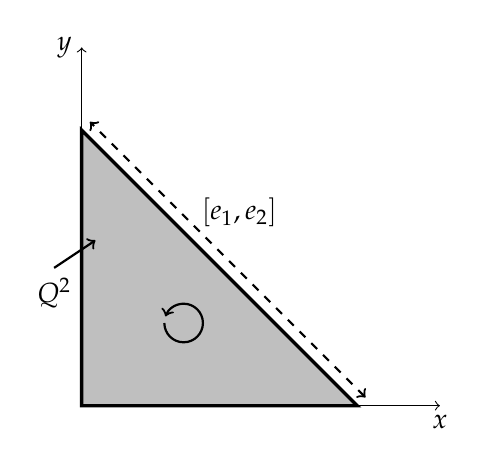
\begin{tikzpicture}[scale=3.5]
	\draw[->] (0,0)--node[below,pos=1]{$x$}(1.3,0);
	\draw[->] (0,0)--node[left,pos=1]{$y$}(0,1.3);
	\draw [very thick,fill=gray,fill opacity=.5](0,0)--(1,0)--(0,1)--cycle;
	\draw [thick,->](-0.1,0.5)--node[below,pos=0]{$Q^2$}(0.05,0.6);
	\draw [thick,dashed,<->](1.03,0.03)--(0.03,1.03);
	\node[right] at (0.4,0.7) {$[e_1,e_2]$} ;
	\draw[thick,->] (0.3,0.3) arc [start angle = -180, end angle = 160, radius=0.07];
\end{tikzpicture}

&& now for similar case in $\R^3$ : consider a $3$-simplex $Q^3=[0,e_1,e_2,e_3]$ in $\R^3$ : it forms trigonal pyramid or a filled tetrahedron like structure here the 'boundary' of the figure are 4 triangular surfaces (filled or area vise) these are just $2$-simplexes like the one in $xy$-plane is just $[0,e_1,e_2]$, so the whole boundary can be represented as a affine chain $[e_1,e_2,e_3]-[0,e_2,e_3]+[0,e_1,e_3]-[0,e_1,e_2]$ 

\end{easylist}

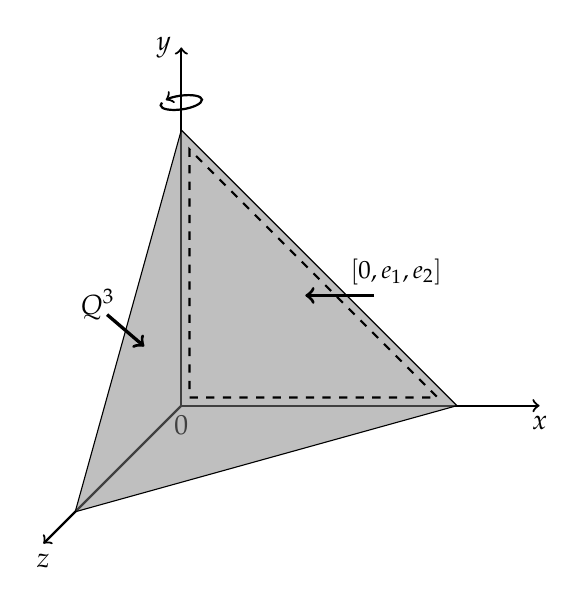
\begin{tikzpicture}[scale=3.5]
	\node[below] at (0,0,0) {$0$};
	\draw[thick,->] (0,0,0) -- node [below, pos=1]{$x$}(1.3,0,0);
	\draw[thick,->] (0,0,0) -- node [left, pos=1]{$y$}(0,1.3,0);
	\draw[thick,->] (0,0,0) -- node [below, pos=1]{$z$}(0,0,1.3);
	\draw[thin,fill=gray,fill opacity=.5] (1,0,0)--(0,1,0)--(0,0,1)--cycle;
	\begin{scope}[canvas is xy plane at z=0]
		\draw[dashed,thick,] (0.03,0.03)--(0.93,0.03)--(0.03,0.93)--cycle;
		\draw[very thick,->] (0.7,0.4)--node[above right]{\small$[0,e_1,e_2]$}(0.45,0.4);
	\end{scope}
	\begin{scope}[canvas is zy plane at x=0]
%		\draw[dotted,thick] (0.05,0.07)--(0.85,0.07)--(0.05,0.85)--cycle;
		\draw[very thick,->] (0.7,0.6)--node [above left]{$Q^3$}(0.35,0.35);
	\end{scope}
	\begin{scope}[canvas is xz plane at y=1.1]
		\draw[thick,->] (-0.07,0) arc  [start angle =180, end angle = -160, radius=0.07];
	\end{scope}
\end{tikzpicture}

\begin{easylist}
	& generalizing this we get for $k\geq 1$ the\textbf{ boundary of the oriented affine $k$-simplex } $\sigma=[p_0,p_1,\ck,p_k]$ is defined to be the $(k-1)$-chain 
	\begin{center}
		$\partial\sigma=\sm{j=0}{k}(-1)^j[p_0,\ck,p_{j-1},p_{j+1},\ck,p_k]$
	\end{center}
	(note the sign or $j$ depends on removal $j$th position not on $j$th index as indexes may be rearranged)
& \textbf{oriented $k$-simplex} of class $\mathscr{C}''$ : if $T$ is a $\mathscr{C}''$ map of an open set $E\subset\R^n$ into a open set $V\subset \R^m$,$\sigma$ an oriented affine $k$-simplex in $E$ then $\Phi=T\circ \sigma=T\sigma$ is a $k$-surface in $V$ with parameter domain $Q^k$ this $\Phi$ is called oriented $k$-simplex of class $\mathscr{C}''$ i.e. $\Phi:Q^k\xrightarrow{T\sigma}V$
& a finite collection $\Psi$ of oriented $k$-simplexes $\Phi_1,\ck,\Phi_r$ of class $\mathscr{C}''$ in $V$ is a defined as\textbf{ $k$-chain of class $\mathscr{C}''$ }in $V$
&& if $\omega$ is $k$-form in $V$ then we define 
\begin{center}
	$\int_{\Psi}\omega=\sm{i=1}{r}\int_{\Phi_i}{\omega}$ 
\end{center}
and we use the corresponding notation $\Psi=\sum\Phi_i$ 
&& iif $\Gamma=\sum\sigma_i$ is an affine chain and $\Phi_i=T\circ\sigma_i$ we also write $\Psi=T\circ\Gamma$ or $T(\sum\sigma_i)=\sum T\sigma_i$
&& Boundary $\partial\Phi$ of the oriented $k$-simplex $\Phi=T\circ\sigma$ is defined to be $k-1$ chain $\partial\Phi=T(\partial\sigma)$
&& Boundary of $k$-chain $\Psi=\sum\Phi_i$ is defined as $k-1$-chain $\partial\Psi=\sum \partial\Phi_i$
& eg: unit square $I^2\subset \R^2$ is union of $\sigma_1(Q^2)$ and $\sigma_2(Q^2)$ where $\sigma_1(u)=u$ i.e. $\sigma_1=[0,e_1,e_2]$ and $\sigma_2(u)=e_1+e_2-u=$ i.e. $\sigma_2=[e_1+e_2,e_2,e_1]$ so \\
$\partial\sigma_1=[e_1,e_2]-[0,e_2]+[0,e_1]$\\
$\partial\sigma_2=[e_2,e_1]-[e_1+e_2,e_1]+[e_1+e_2,e_2]$ so the sum of boundaries are $\partial I^2=\partial\sigma_1+\partial\sigma_2\\
=[0,e_1]+[e_1,e_1+e_2]+[e_1+e_2,e_2]+[e_2,0]$ which is the positively oriented boundary of $I^2$ now if $\Phi$ is a $2$-surface in $\R^m$ with parameter domain $I^2$ then it is same as $2$-chain $\Phi\circ\sigma_1+\Phi\circ\sigma_2$ thus $\partial\Phi=\Phi(\partial\sigma_1)+\Phi(\partial\sigma_2)=\partial\Phi(\partial I^2)$ so decomposition of $I^2$ into simplexes is can be neglected and $\partial\Phi$ can be directly obtained from $\partial I^2$
& \textbf{\Large Stokes' Theorem} (generalized fundamental theorem of calculus): if $\Psi$ is a $k$-chain of class $\mathscr{C}''$ in an open set $V\subset \R^m$ and $\omega$ a $k-1$-form of class $\mathscr{C}'$ in $V$ then \[\int_{\Psi}{d\omega}=\int_{\partial\Psi}{\omega}.\] 
& for $\omega$ a $k$-form in open set $E\subset\R^k$ :
&& if there is a $k-1$-form $\lambda$ in $E$ such that $\omega=d\lambda$ then $\omega$ is called an \textbf{Exact form} in $E$
&& if $\omega$ is of class $\mathscr{C}'$ and $d\omega=0$ then $\omega$ \textbf{Closed form} in $E$
& clearly if $\omega$ is class $\mathscr{C}'$ and exact then it is closed.
& a give $1$-form $\omega=\sm{i=1}{n}f_i(x)dx_i$ is closed in $E$ iff $(D_jf_i)(x)=(D_if_j)(x) \, \forall x\in E$ 
& for $\omega$ is exact $k$-form in $E$ then $\omega=d\lambda$ and by stokes theorem we have\\ $\int_{\Phi}\omega=\int_{\Phi}d\lambda=\int_{\partial\Phi}\lambda$ for every $k$-chain $\Phi$ \\
thus $\int_{\Phi_1}\omega=\int_{\Phi_2}\omega.$ if $\Phi_1$ and $\Phi_2$ have same boundaries\\
in particular the integral is zero over every $k$-chain in $E$ whose boundary is zero, so integrals of exact $1$-forms in $E$ are $0$ over closed differentiable curves in $E$
& if $\omega$ is a closed form in $E$ then by stokes theorem \\
$\int_{\partial\Phi}\omega=\int_{\Phi}d\omega=0.$ for every $k+1$-chain $\Phi$ in $E$
& \textbf{In a convex set closed forms are exact} (note form is of class $\mathscr{C}'$ is assumed)
& now if $T$ is 1-1 $\mathscr{C}''$ map of $E\subset \R^n$ onto $U\subset \R^n$ such that $T^{-1}=S$ is also $\mathscr{C}''$ and if every closed form is exact in $E$ or $E$ is open convex set i.e. 
for convex open $E\underset{\xleftarrow[S=T^{-1} \,\mathscr{C}''\w{map} ]{ }}
{\xrightarrow{T \,\w{bijective, }\mathscr{C}''\w{map}}} U $ then
every closed form in $U$ is exact \\
if $E$ and $U$ are as in assumption of above then we say $U$ is $\mathscr{C}''$-equivalent to $E$.\\
\ckfil
\end{easylist}
\begin{easylist}
\section{Vector Analysis and Forms}
& \textbf{Vector Field} $F:E\subset\R^3\ra\R^3$ is a continuous mapping in which $F$ associates each point $x\in E$ to a vector\\ $F_1(x)e_1+F_2(x)e_2+F_3(x)e_2=(F_x,F_y,F_z)$ (note $F_1=F_x,F_2=F_y,F_3=F_z$ only mere notation changes)
& we can associate $1$-form and $2$-form to $F=F_1e_1+F_2e_2+F_3e_3$ (vector field) as
&& $\lambda_F=F_1dx+F_2dy+F_3dz.$
&& $\omega_F=F_1dy\land dz+F_2dz \land dx+F_3dx\land dy.$
& \textbf{Gradient} : for real function $u\in \mathscr{C}'(E)$, $E\subset\R^3 $
\begin{center}
	$\nabla u=\pfrac{u}{x_1}e_1+\pfrac{u}{x_2}e_2+\pfrac{u}{x_3}e_3=(\pfrac{u}{x},\pfrac{u}{y},\pfrac{u}{z})$
\end{center}
& for Vector field $F\in \mathscr{C}'(E)$ :
& \textbf{Divergence} of $F$: is a real function defined by \begin{center}
	$\nabla . F=\pfrac{F_1}{x_1}+\pfrac{F_2}{x_2}+\pfrac{F_3}{x_3}
	=\pfrac{F_x}{x}+\pfrac{F_y}{y}+\pfrac{F_z}{z}$\end{center}
& \textbf{Curl} of $F$: is again a vector field given by the determinant 

\end{easylist}
$\nabla\times F=
\begin{vmatrix}
	e_1 & e_2 & e_3 \\
	\pfrac{ }{x_1} & \pfrac{ }{x_2} & \pfrac{ }{x_3} \\
	F_1 & F_2 & F_3 \\
\end{vmatrix}
=
\begin{vmatrix}
	e_1 & e_2 & e_3 \\
	\pfrac{ }{x} & \pfrac{ }{y} & \pfrac{ }{z} \\
	F_x & F_y & F_z \\
\end{vmatrix}$
\begin{easylist}
where determinant is expanded from 1st row, $\pfrac{ }{x_i}F_j=\pfrac{F_j}{x_i}$ or $\pfrac{ }{x}F_z=\pfrac{F_z}{x}$ and like wise
& basic properties (can be derived by associating appropriate forms to vector fields)
&& if $F=\nabla U$ then $\nabla \times F=0$
&& if $F=\nabla \times G$ then $\nabla.F=0$
further if $ $
&& if $E$ is convex or $\mathscr{C}''$-equivalent to a convex set then converse of above point holds i.e.
&& if $\nabla \times F=0$ then $F=\nabla U$ for some real function $U$ in $E$
&& if $\nabla.F=0$ then $F=\nabla \times G$ for some vector field $G$ in $E$
\end{easylist}
\subsection{Consequences of Stokes' Theorem}
\begin{easylist}
& \textbf{Greens Theorem} : for open $E\subset \R^2$ and $\alpha,\beta\in \mathscr{C}'(E)$, and for a closed set $\Omega$ of $E$ with positively oriented boundary $\partial\Omega$ then 
\[\int_{\partial\Omega}{\alpha dx+\beta dy}=\int_{\Omega}{\left(\pfrac{\beta}{x}-\pfrac{\alpha}{y}\right)dA}\]
where $dA=dx\land dy$\\
(use $\alpha dx+\beta dy$ as $1$-form)
& \textbf{Area element} in $\R^3$ for $\Phi$ a $2$-surface in $\R^3$ of class $\mathscr{C}'$ with parameter domain $D\subset \R^2$ associate each point $(u,v)$ vector 
\begin{center}
	$N(u,v)=\pfrac{(y,z)}{(u,v)}e_1+\pfrac{(z,x)}{(u,v)}e_2+\pfrac{(x,y)}{(u,v)}e_3$ 
\end{center}
for Jacobians defined on $(x,y,z)=\Phi(u,v)$
&& if $f$ is continuous on $\Phi(D)$ then the area integral of $f$ over $\Phi$ is defined to be 
\begin{center}
	$\int_{\Phi}{fdA}=\int_{D}{f(\Phi(u,v))|N(u,v)|dudv}$
\end{center}
this makes sense as $N$ is perpendicular to tangent planes and $|N|$ is the area of small parallelogram below $N$ on surface $\Phi$ (all when $\Phi$ is considered locally an affine map).
& Integral of $1$-forms in $\R^3$ : if $\gamma$ is a $\mathscr{C}'$-curve in an open set $E\subset\R^3$ with parameter interval $[0,1]$, $F$ a vector field in $E$ then for tangent vector 
$\gamma '(u)=\gamma_1'(u)e_1+\gamma_2'(u)e_2+\gamma_3'(u)e_3=|\gamma'(u)|t(u)$ where $t(u)$ is defined as unit tangent vector in $\gamma'(u)$ direction, we have
\end{easylist}
{\small
\begin{align*}
	\int_{\gamma}{\lambda_F}& =\sm{i=1}{3}\int_{0}^{1}F_i(\gamma(u))\gamma'(u)du\\
	& \qquad\w{\small (from definition of $1$-form)}\\
	& =\int_{0}^{1}F(\gamma(u)).\gamma'(u)du\\
	& =\int_{0}^{1}(F.t)ds
\end{align*} }
where $ds=|\gamma'(u)|du$ is the element of arc length along $\gamma$
\begin{easylist}
& Integral of $2$-forms in $\R^3$ : if $\Phi$ is a $2$-surface of class $\mathscr{C}'$ in an open set $E\subset\R^3$ with parameter domain $D\subset\R^2$, $F$ a vector field in $E$ then 
\end{easylist}
{\small
\begin{align*}
	\int_{\Phi}{\omega_F}& ={\int_{\Phi}F_1dy\land dz+F_2dz \land dx+F_3dx\land dy}\\
	& \qquad\w{\small (from definition of $1$-form)}\\
	& =\int_{D} \left[F_1\circ \Phi \pfrac{(y,z)}{(u,v)}+F_2\circ \right. \Phi\pfrac{(z,x)}{(u,v)}\\
	& \quad \left. +F_3\circ \Phi\pfrac{(x,y)}{(u,v)}  \right] dudv\\
	& = \int_{D}F(\Phi(u,v)).N(u,v)dudv \\
	& = \int_{D}F(\Phi(u,v)).n(u,v)|N(u,v)|dudv \\
	& = \int_{D}(F.n) dA\\
\end{align*} }
where $n(u,v)$ is the unit vector along $N(u,v)$ and $dA=|N(u,v)|dudv$ is the area element on $\Phi$ 
\begin{easylist}
& \textbf{Stokes Curl Theorem} : for $F$ vector field of class $\mathscr{C}'$ in open set $E\subset\R^3$ and if $\Phi$ is $2$-surface of class $\mathscr{C}''$ in $E$, then 
\[\int_{\Phi}(\nabla\times F).ndA=\int_{\partial\Phi}{F.t}ds.\]
(direct consequence of Stokes' Theorem)
& \textbf{Gauss Divergence Theorem} : for $F$ vector field of class $\mathscr{C}'$ in open set $E\subset\R^3$ and if closed $\Omega\subset E$ has a positive oriented boundary $\partial \Omega$ then 
\[\int_{\Omega}{\nabla.F}dV=\int_{\partial\Omega}{(F.n)dA}.\]
(direct consequence of Stokes' Theorem)
& \textbf{Generalized Integration by parts} :
&& Integration by parts : if $F,G$ are differentiable functions on $[a,b]$, $F'=f\in \mathscr{R}$ and $G'=g\in \mathscr{R}$ then
\end{easylist}
{\small
\begin{align*}
\int_{a}^{b}F(x)g(x)dx & =F(b)G(b)-F(a)F(a)\\
& \qquad -\int_{a}^{b}f(x)G(x)dx
\end{align*}}
\begin{easylist}
&& \textbf{Generalized version } : for open set $E\subset\R^n$,$k$-form $\omega$ of class $\mathscr{C}'(E)$, $f$ real function of class $\mathscr{C}'(E)$ and $\Phi$ a $k$-surface of class $\mathscr{C}''$ in $E$ then 
\[\int_{\Phi}fd\omega=\int_{\partial\Phi}{f\omega}-\int_{\Phi}{(df)\land\omega}\]
\ckfil
\section{Lebesgue Integration \\ and measures}
& \textbf{ring} (not the same as abstract but is relevant) : a family of sets $ \mathfrak{R} $ is a ring if $ A\in \mathfrak{R}, \, B \in \mathfrak{R} $ implies
\begin{center}
	$ A\cup B \in \mathfrak{R},\,A-B \in \mathfrak{R}.$
\end{center}
(note $ A\cap B =A-(A-B) $ so  $ A\cap B \in \mathfrak{R} $)
& \textbf{$\sigma$-ring} : $\mathfrak{R}$ is a $ \sigma $-ring if it a ring with 
property that if $ A_n \in \mathfrak{R} $ then 
\begin{center}
	$ \displaystyle \cup_{i=1}^{\infty}A_n \in \mathfrak{R}.$
\end{center}
(note $ \displaystyle \cap_{i=1}^{\infty}A_n \in \mathfrak{R}.$)
& \textbf{Set function} $ \phi:\mathfrak{R}\ra \R+{\infty} $ i.e. $\phi $ maps sets in a ring to extended real line 
&& $ \phi $ is additive if $ A\cap B=0 $(empty set) implies 
\begin{center}
	$ \phi(A\cup B)=\phi(A)+\phi(B) .$
\end{center}
&& $ \phi $ is countably additive if $ A_i\cap A_j=0 $ implies 
\begin{center}
	$ \phi(\cup_{i=1}^{\infty}A_i)=\sm{i=1}{\infty}\phi(A_i).$
\end{center}
& properties of additive set function $ \phi $ :
&& $ \phi(0)=0. $
&& $ \phi(A_1\cup\ck\cup A_n)=\phi(A_1)+\ck +\phi(A_n) .$ 
for $ A_i\cap A_j=0(i\neq j) $
&& $ \phi(A_1\cup A_2)+\phi(A_1\cap A_2)=\phi(A_1)+\phi(A_2) .$
&& if $ \phi(A)\geq 0\, \forall A\in \mathfrak{R}$ then we say $ \phi  $ is nonnegative, now for such $ \phi $ (also additive) if $ A_1\subset A_2 $ then 
\begin{center}
	$ \phi(A_1)\leq \phi(A_2).$
\end{center}
&& if $ \phi  $ is non-negative, additive and $ B\subset A\in \mathfrak{R}(\phi(B)<\infty) $ then
\begin{center}
	$ \phi(A-B)=\phi(A)-\phi(B) .$
\end{center}
& if $ \phi $ is countably additive on ring $ \mathfrak{R} $, $ A_n\in \mathfrak{R} ,\, A_1\subset A_2 \subset\ck ,A\in \mathfrak{R}$ such that $ A=\cup_{i=1}^\infty
A_i$ then 
\begin{center}
	$ \phi(A_n)\ra \phi(A) .$
\end{center}
\subsection{Formation of Lebesgue measures on $\R^p$}
& \textbf{ Interval } in $ \R^p $: is just a bounded $ k $-cell or $\{(x_1,\ck ,x_n):a_i\leq x_i \leq b_i,\, \{a_i,b_i\}\subset\R\}$ (note $ a_i,b_i\neq \pm\infty $)
and in any $ \leq $ is replaced with $ < $ is also an intrval and the case $ a_i=b_i $ is ruled out 
& \textbf{Elementary set} : a set which is the union of finite intervals 
& example: define  $ m(I) $ for interval $ I \subset \R^p$ as $ m(I)=\prod_{i=1}^p(b_i-a_i) $
then for $ \mathscr{E} $ family of all Elementary subset of $ \R^p $ we have :
&& $ \mathscr{E} $ is ring but not $ \sigma $-ring (as countale intersection of closed Intervals may be finite sets)
&& if $ A\in \mathscr{E} $ then $ A $ is the finite union of disjoint Intervals
&& $ m $ is a non-negative additive set function on $ \mathscr{E} $\\
( clearly if $ p=1,2,3 $ then $ m $ is just length, area , volume)
& A non-negative additive set function $ \phi  $ on $ \mathscr{E} $ is regular if
for each $\epsilon>0$  $, A\in \mathscr{E}\;\exists F,G\in \mathscr{E} $ such that
$ F $ closed , $ G $ open , $ F\subset A\subset G $ and 
\begin{center}
	$ \phi(G)-\epsilon \leq \phi(A) \leq \phi(F)+\epsilon .$
\end{center}
i.e. $ \phi(A) $ can be taken as a limit of $ \phi $ in open superset or closed subset of $ A .$
& $ m $ is regular 
& \textbf{outer measure} : $ \mu^* $ for a additive, nonnegative, regular and finite on $ \mathscr{E} $ in $ \R^p $, for countable covering of $ E\subset\R^p $ by open Elementary sets $ A_n $ i.e. $ E\subset \cup_{n=1}^\infty A_n .$ then define 
\begin{center}
	$ \mu^*(E)=\inf \sm{n=1}{\infty}\mu(A_n) .$
\end{center} 
(one similarly define inner measure as supremum of disjoint closed elementary subsets contained in $ A $ and can construct Lebesgue measure also but the measure obtained is same for a given $ \mu $)
& properties of outer measure :
&& for every $ A\in \mathscr{E},\, \mu^*(A)=\mu(A) $ i.e. outer measure is just an extension of $ \mu $ 
&& if $ E=\cup_1^\infty E_n $ then $ \mu^*(E)\leq \sm{1}{\infty}\mu^*(E_n) $ i.e.
$ \mu^* $ is sub-additive.
& \textbf{Symmetric difference} $ S(A,B) $ : $ A,B\in \R^p\; S(A,B)=(A-B)\cup (B-A) $
& define $ d(A,B)=\mu^*(S(A,B)) $ and $ A_n \ra A $ if $ \lim\limits_{n\ra \infty}
d(A,A_n)=0 $ for sequence of elementary sets $ \{A_n\} $.
& $ \mathfrak{M}_F(\mu) $ contains sets $ A $ (finitely $ \mu $ measurable) if there exist elementary set sequence $ \{A_n\} $ such that $ A_n\ra A $
(i.e. $ \lim\limits_{n\ra \infty}d(A,A_n)=0 $ )
& $\mathfrak{M}(\mu) $ contains all sets that are countable union of finitely $ \mu $-measurable sets.
& \textbf{Measure theorem } on Euclidean space : $ \mathfrak{M}(\mu) $ is a $ \sigma $-ring and $ \mu^* $ is countable additive.
& such extended set function (nonnegative, countably additive, regular and finite) 
on $ \sigma $-ring is called as \textbf{measure} 
& \textbf{Lebesgue measure} $ m $ is extension of set function $ m $ (defined earlier) on
$ \sigma $-ring $ \mathfrak{M}(m) $ in $ \R^p $.
& properties of  measures :
&& if $ A $ is open or closed in $ \R^p $then $ A\in \mathfrak{M}(\mu) $ (as $ \R^p $ has a countable base consisting of only open intervals)
&& if $ A\in \mathfrak{M}(\mu) $ and for every $ \epsilon >0 $ there exist sets :
closed $ F $ and open $ G $ such that $ F\subset A\subset G $ and 
\begin{center}
	$ \mu(G-A)<\epsilon ,\, \mu(F-A)<\epsilon .$
\end{center}
&& \textbf{Borel sets} : sets which are countable union, intersection or complement union or intersection of open sets, clearly the collection $ \mathscr{B} $ of all 
Borel sets in $ \R^p $ is the smallest $ \sigma $-ring containing all open sets and
$ \mathscr{B}\subset \mathfrak{M}(\mu) $
& relevance to Riemann integration

&& if $ A\in \mathfrak{M}(\mu) $ and for every $ \epsilon >0 $ there exist Borel sets $ F, G $ such that $ F\subset A\subset G $ and 
\begin{center}
	$ \mu(G-A)=\mu(F-A)=0.$
\end{center}
&& Thus $ A\in \mathfrak{M}(\mu) $ then $ A=F\cup (A-F) $ where $ F $ is Borel set and $ A-F $ is a set of measure zero
&& for a given $ \mu $ Borel sets are same but sets of measure zero may differ

\subsection{Measure Space}
& $ X $ is a measure space if there exist a $ \sigma  $-ring $ \mathfrak{M} $ of subsets of $ X $ (which are called measurable sets) and a nonnegative countably additive set function  $ \mu $ (called measure) defined on $ \mathfrak{M} $
& \textbf{Measureable Function} : a function $ f $ defined on measure space $ X $
to extended Reals such that the sets $ \{x:f(x)>a\} $ is measurable for every real $ a $
& this definition is equivalent to 
\begin{center}
	$ \{x:f(x)\geq a\} .$\\
	$ \{x:f(x) < a\} .$\\
	$ \{x:f(x) \leq a\} .$
\end{center}
& if $ f,g $ are measurable on $ X $ then :
&& $ |f| $ is measurable
&& $ max(f,g),\, min(f,g) $ are measurable
&& $ f=f^+-f^- $ where $ f^+=max(f,0),f^-=min(f,0) \geq 0 $ are measurable.
&& if $\{f_n\}$ is sequence of measurable functions then $ h(x)=\sup f_n(x) (1,\ck ,n) $ and $ k(x)=\limsup_{n \ra \infty}f_n(x) $ are Measureable
& If $ F $ is continuous function on $ \R^2 \ra \R $ , and $ f,g $ are measurable then 
\begin{center}
	$ h(x)=F(f(x),g(x)) .$ 
\end{center} is measurable. ( in particulat $ f+g(x),f(x)g(x) $ are measurable)
& \textbf{Characteristic function} 
\end{easylist}

$ K_E(x)= 
\begin{cases}
	1 & \quad (x\in E)\\
	0 & \quad (x \notin E)
\end{cases} $

\begin{easylist}
is measurable iff $ E $ is measurable
& \textbf{Simple function} $ s $ : a functions with finite range \\
if range of $ s $ consists of distinct numbers $ c_1,c_2,\ck,c_n $,if 
$ E_i=\{x_i:s(x_i)=c_i\} $ then 
\begin{center}
	$ s=\sm{i=1}{\infty}c_i K_{E_i} .$
\end{center}
and $ s $ is measurable if each $ E_i $ is measurable.
& for every real function $ f $ on measure space $ X $ there exist as sequence of
simple functions $ \{s_n\} $ such that $ s_n(x)\ra f(x) $ as $ n\ra \infty $

\subsection{Lebesgue Integration}
& for a given measure $ \mu $ and measurable simple function $ s=\sm{i=1}{\infty}c_i K_{E_i}$ we define 
\begin{center}
	$ \int_{E}s d\mu = \sm{i=1}{\infty} c_i \mu(E\cap E_i) .$
\end{center}
& if $ f $ is nonnegative measurable function then for $ 0\geq s\geq f$ ($s $ simple) define
\begin{center}
	$ \int_E fd\mu= \sup \int_E sd\mu .$
\end{center}
& if $f$ is in general (positive aswell as negative) measurable then 
$ f= f^+ - f^- $ and define 
\begin{center}
	$ \int_E fd\mu = \int_E f^+ d\mu - \int_E f^- d\mu .$
\end{center}
& we say a measurable function $ f $ is Lebesgue integrable on $ E $ or 
$ f\in \mathscr{L}(\mu) $ on $ E $ if its Lebesgue integral is finite on $ E $

& properties of Lebesgue integrable Functions
&& if $ a\leq f(x)\leq b $ on $ E $ and $ \mu(E)< \infty $ then 
\begin{center}
	$ a\mu(E)\leq \int_E fd\mu \leq b\mu(E) .$
\end{center}
&& if $ f,g \in \mathscr{L}(\mu) $ on $ E $ and $ f\leq g $ on $ E $ then 
\begin{center}
	$ \int_E f d\mu \leq \int_E g d\mu .$
\end{center}
&& for any real (constant) $ c $ if $f\in \mathscr{L}(\mu)$ on $E$ then $ cf \in \mathscr{L}(E) $ and $ \int_E cfd\mu = c\int_E fd\mu $
&& if $ \mu(E)=0 $ then for measurable $ f,\int_E f d\mu =0.$ 
&& if $f\in \mathscr{L}(\mu)$ on $ E $ and measurable $A\subset E$ then $ f \in \mathscr{L}(\mu) $ on $ A $
& for measurable, nonnegative $ f $ on $X$ and a measurable set $ A\subset X $ define $ \phi(A)= \int_A fd\mu $ then $ \phi $ is countably additive on measurable sets
i.e. for a sequence $ \{ A_n\} $ of measurable sets
\begin{center}
	$ \int_{A_1\cup A_2\cup \ck} fd\mu =\int_{A_1} fd\mu +\int_{A_2}f d\mu .$
\end{center}
& if $A,B\in \mathfrak{M}, B\subset A$ and $ \mu(A-B)=0 $ then $ \int_A fd\mu=\int _B fd\mu .$
& \textbf{almost everywhere} : excluding sets of measure zero i.e. \\
eg: if $ f=g $ almost everywhere if $ \{x:f(x)\neq g(x)\}\cap E $ has measure zero
& if $ f\in \mathscr{L}(\mu) $ on $ E $ then $ |f|\in \mathscr{L})(\mu) $ on $ E $
and
\begin{center}
	$ \left|\int_E f d\mu \right| \leq \int_E |f| d\mu .$
\end{center}

& if $ f $ measurable on $ E $, $ |f|\leq g $ and $ g\in \mathscr{L}(\mu) $ on $ E $ then $ f\in \mathscr{L}(\mu) $ on $ E $
& \textbf{Lebesgue monotone convergence theorem} : for $ E\in \mathfrak{M} $ and 
$ \{f_n\} $ a sequence of measurable functions such that $ 0\leq f_1(x)\leq f_2(x)
\ck $ on $ E $, if $ f_n \ra f $ as $ n\ra \infty $ on $ E $ then as $n\ra \infty$
\begin{center}
	$ \int_E f_n d\mu \ra \int_E fd\mu .$
\end{center}
& Consequences 
&& if $ f_1,f_2\in \mathscr{L}(\mu) $ on $ E\in \mathfrak{M}$ then $ f_1+f_2 \in \mathscr{L}(\mu)$on $ E $
&& if $ \{f_n\} $ is a sequence of nonnegative measurable functions on
$ E  \in \mathfrak{M}$ and $ f(x)=\sum f_n(x) $ on $ E $ then 
\begin{center}
	$ \int_E fd\mu=\sum \int_E f_n d\mu .$
\end{center}
& \textbf{Fatou's Theorem} : if $ \{f_n\} $ is a sequence of nonnegative measurable functions on $ E\in   \mathfrak{M}$ and 
$ f(x)=\liminf_{n\ra \infty} f_n(x) $ on $ E $ then 
\begin{center}
	$ \int_E fd\mu \leq \liminf_{n\ra \infty} \int_E f_n d\mu .$
\end{center}

& \textbf{Lebesgue Dominated convergence Theorem} : if $ \{f_n\} $ is a sequence of
nonnegative measurable functions on $ E\in  \mathfrak{M}$,
$  f_n(x) \ra f(x) $ on $ E $ and if there exist $g\in \mathscr{L}(\mu)  $ on 
$ E $ such that $ |f_n(x)|\leq g(x)\, \forall n $ on $ E $ then 
\begin{center}
	$ \lim\limits_{n\ra \infty} \int_E f_n d\mu = \int_E f d\mu .$
\end{center}

& on Interval $ [a,b] $ if $ f\in \mathscr{R} $ then $ f \in \mathfrak{L}(m) $ on the interval and 
\begin{center}
	$ \int_{[a,b]}f dm = \int_a^b f dx .$
\end{center} (note $m$ is the Lebesgue measure)
& most theorems like fundamental theorem of calculus hold for Lebesgue integration with measure $ m $\\
\ckfil
\end{easylist}
\begin{thebibliography}{9}
	\bibitem{Ru}
	Rudin W.: Principles of Mathematical Analysis, McGraw-Hill, 3, (1976).
	\bibitem{BT}
	Robert G. Bartle, Donald R. Sherbert: Introduction to Real Analysis, Wiley publishers, 4, (2011).
\end{thebibliography}
\end{multicols}
\end{document}
